\chapter{形式理论}
本节我们介绍更适合描述量子力学的数学语言，我们的讨论从一维无限深势阱出发. 考虑势能：
\[
U = 
\begin{cases}
0 & 0\leq x \leq a \\
\infty & \mathrm{else}
\end{cases}
\]
这时，定态Schrodinger方程写为：
\[
-\frac{\hbar^2}{2m}\frac{\dd^2\psi}{\dd x^2} = E\psi
\]
同时，由于两侧势垒为无穷大，因此粒子穿过概率为0，因此
\[
\psi(0) = \psi(a) = 0
\]
这时，问题转化为Sturm-Liouville本征值问题，因此求解得到解：
\[
\psi_{n}(x) = A_{n}\sin\frac{n\pi}{a}x
\]
其中
\[
E_{n} = \frac{n^2\pi^2\hh^2}{2ma^2}
\]
因此，含时Schrodinger方程的解为：
\[
\Psi(x,t) = \sum_{n}c_{n}\psi_{n}\exp(-i\frac{n^2\pi^2\hh}{2ma^2}t)
\]
要求解系数\(c_{n}\)，我们想到偏微分方程的Fourier技巧：取\(t=0\)时刻，两边乘定态波函数的共轭\(\psi^{*}\)，做积分，得到：
\[
c_{n}\int_{0}^{a}\psi_{n}^{*}\psi_{n}\dd x = \int_{0}^{a}\Psi(x,0)\psi_{n}^{*}(x)\dd x
\]
带入本情景下的\(\psi_{n}\)，得到：
\[
c_{n} = \frac{2}{A_{n}^{2}a}\int_{0}^{a}\Psi(x,0)\psi_{n}^{*}(x)\dd x
\]
为了结果的简洁，我们令\(\frac{2}{A_{n}^{2}a}=1\)，所以有
\[
\psi_{n}(x) = \sqrt{\frac{2}{a}}\sin\frac{n\pi}{a}x
\]
此时，定态波函数被归一化. 回顾求解的过程，我们实际上做的是这样几件事情：
\begin{itemize}
    \item 时间空间因子分立，得到本征方程，求解本征函数. 
    \item 归一化本征函数.
    \item 用本征函数列的无穷级数表示完整解，利用初始条件确定系数. 
\end{itemize}
我们再看线性代数中的一个问题，考虑一个矩阵\(\mathbf{A}\)，满足：
\[
\mathbf{A}
= \begin{bmatrix}
2 & -1 & 0 \\
-1 & 2 & -1 \\
0 & -1 & 2\\
\end{bmatrix}
\]
因此，平面中的向量除开用典型的Cartesian坐标系正交单位基，还能用矩阵A的本征向量描述. 考虑A的本征方程：
\[
\mathbf{A}\mathbf{v} = \lambda\mathbf{v}
\]
求解
\[
\det(\mathbf{A}-\lambda\mathbf{I}) = 0
\]
得到
\[
\lambda_{1} = 2 , \lambda_{2} = 2+\sqrt{2}, \lambda_{3} = 2-\sqrt{2}
\]
所以，三个本征向量为：
\begin{align*}
& \mathbf{v}_{1} = \frac{1}{\sqrt{2}}(1, 0, -1)^{T} \\
& \mathbf{v}_{2} = \frac{1}{2}(1, -\sqrt{2}, 1)^{T} \\
& \mathbf{v}_{3} = \frac{1}{2}(1, \sqrt{2}, 1)^{T}
\end{align*}
这时，空间中任意一个向量\(\mathbf{u}\)可以被表述为：
\[
\mathbf{u} = \sum_{i}c_{i}\mathbf{v}_{i}
\]
其中，系数等于：
\[
c_{i} = {\mathbf{u}\cdot\mathbf{v}_{i}}
\]
对比两个问题的操作，我们会发现惊人的相似性. 因此，我们完全可以把函数\(\Psi\)看成是向量，\(\psi_{n}\exp(-iE_{n}t/\hh)\)看成是向量的基底，于是，Sturm-Liouville问题就被转化为线性代数里的本征值问题. 由于“函数向量”的基底是无穷多的，所以“函数向量”所在的空间不仅是线性空间，还是Hilbert空间. 我们接下来的讲解讲从Hilbert的来源开始，讨论其完备性，然后引入适合表示Hilbert空间与其运算的Dirac符号，最后我们再讨论其在量子力学的应用. 
\section{Hilbert空间}
我们将视角稍微拉远一点，回顾一下数列与它的极限. 所谓数列，即一组被编号序号的数，数列的极限，就是看序号特别大的时候，这组数的变化有什么特点. 如果数列极限存在，那么这组数彼此间的变化会越来越小，最终在一个确定值附近浮动，记作
\[
\lim_{n\to\infty}x_{n} = a
\]
然后，这种跑动无法被数学语言精确描述，所以我们将“跑动”改为“约束”，即距离的约束给定精度，存在这种序号存在：
\[
\forall\epsilon > 0, \exists N,\mathrm{s.t.}(\ n>N\Longrightarrow \abs{x_{n}-a}<\epsilon)
\]
这种分析方法可以帮助我们严格的描述大部分数列的极限，我们甚至能对不同数学形式的数列有不同的处理方法，如Stolz定理、Toeplitz定理、Heine定理等等. 然而，这些方法要么要求\(x_{n}\)有一个解析的表达式、要么要求\(a\)是先验的，对于一个完全陌生的、未知极限大小的数列，我们的方法是有限的. 具体来说，无非是作差与作比. 为了保证数列极限的平移不变性，我们衡量差，于是有Cauchy审敛定理：
\[
\forall\epsilon>0,\exists N, \mathrm{s.t.}(n,m>N\Longrightarrow\abs{x_{m}-x_{n}}<\epsilon)
\]
于是，我们将相对于极限\(a\)的比较转化为数列内部的两个数相对关系的比较，利用Cauchy审敛原理验证收敛的数列被称为Cauchy列. 数学上可以证明数列有极限和数列是Cauchy列在实数域上的等价性. 但是从证明上看，前者推后者是简单的，而后者反推前者是困难的. 通常，这意味着数列是Cauchy列是一个更宽松的条件. 我们不从数学证明上讨论这一点，我们从直观的例子来展示. 例如，我定义一个空间S，这个空间的元素都是小数. 现在，考虑空间S下的数列\(x_{n}\)，\(x_{n}\)满足：
\[
x_{n} = 1 - (0.1)^{n}
\]
容易发现，数列是Cauchy列的，且极限是\(1\)，但是1不属于空间S，所以数列\(x_{n}\)极限不存在. 于是，我们得到了一个看似荒谬的结论：Cauchy列的极限可以不存在. 相似的例子还有，比如在有理数集Q内讨论数列：
\[
x_{n} = 1.4, 1.41, 1.414, \cdots
\]
最终数列收敛于\(\sqrt{2}\)，又因为\(\sqrt{2}\)不在有理数集内，所以该数列极限不存在. 总结一下会发现，有理数域、自己定义的空间S，都与实数域存在质的差别：数列是Cauchy列和数列极限存在是否是等价命题. 因此，我们定义让Cauchy列极限存在的空间为Hilbert空间，这种“兜得住”的特点，被称为完备性. 当然，Hilbert空间内不只有普通的数字与数列，还有连续的函数，还有其他更抽象的元素，所以我们需要重新定义在Cauchy审敛中\textbf{绝对值}. 首先，最典型的Hilbert空间是复数集\(\mathbb{C}\). 为了完整呈现理论，我们不妨把“几个”实数域纵向“排列”在一起，变成\(\mathbb{C}^{n}\). \(\mathbb{C}^{n}\)是线性空间，在这个线性空间内，还定义了内积：
\[
\langle x,y\rangle = \sum_{i=1}^{n}x^*_{i}y_{i}
\]
基于内积，我们定义了度量——范数：
\[
d = \sqrt{\langle x,x\rangle} = \sqrt{\sum_{i=1}^{n}x_{i}^{*}x_{i}}
\]
所以，推广到所有类型的Hilbert空间，我们都能用类似方法定义度量与内积. 由于量子力学中讨论的是函数，所以我们给出函数内积与范数的定义：
\begin{align*}
& \langle f, g\rangle = \int_{a}^{b}f^{*}(x)g(x)\dd x \\
& \langle f, f\rangle = \int_{a}^{b}\abs{f(x)}^{2}\dd x\\
\end{align*}
需要注意，对于函数这种无穷维的向量，我们需要一定的约束. 这里讨论的是
\[
\int_{a}^{b}|f(x)|^{2}\dd x<\infty
\]
的函数f，这是为了保证概率波的归一化可行. 
\section{Dirac符号}
本节，我们将视角放在\textbf{内积}上. 什么是内积？内积就是输入两个向量输出一个数. 这时，我们可以把输入的向量和作用合一起看作映射：
\[
\langle f,\cdot\rangle
\]
所有这些元素在一起构成\textbf{对偶空间}. 它描述的是，与线性空间伴生的，作用于线性空间输出数的空间. 例如，波矢所在空间是位矢所在空间的对偶空间，两个空间内的元素定义了内积：
\[
\phi = k_{\mu}x^{\mu} = -\omega t + \vk\cdot\mathbf{x}
\]
同理，一个列向量的共轭转置(\((a_{i}^{*})^{T}\triangleq a^{\dagger}\))构成的空间是原列向量张成空间的对偶空间：
\[
a^\dagger a = \sum_{i}a^{*}_{i}a_{i}
\]
对偶空间本身的特点是单射反线性. 数学名词很复杂，解释起来就是，对偶空间内的元素不一定能完全映射回原空间. 原本的线性空间和对偶空间的关系可以用图\ref{The_relation_between_the_Linear_Space_and_its_CP}表示. 
\begin{figure}
    \centering
    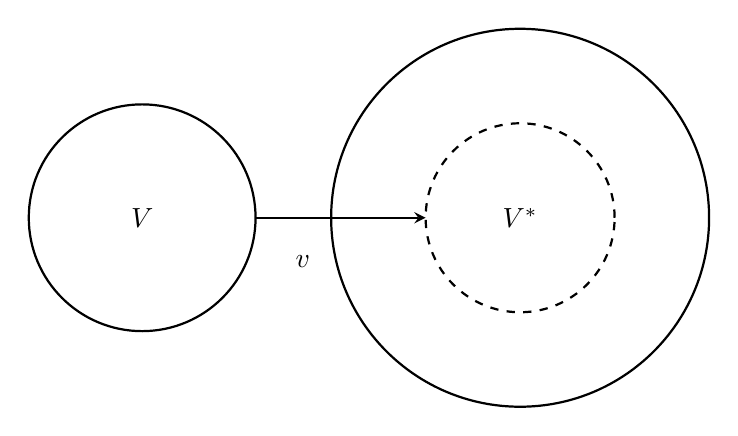
\begin{tikzpicture}[
    >=stealth,
    scale=1.2
]
    % 左侧圆和文字
    \draw[thick] (0,0) circle (1.2) node {$V$};
    
    % 右侧大圆
    \draw[thick] (4,0) circle (2);
    % 右侧虚线圆
    \draw[thick, dashed] (4,0) circle (1) node {$V^*$};
    
    % 箭头与标签
    \draw[thick, ->] (1.2,0) -- (3,0);
    \node[below] at (1.7, -0.3) {$v$};
\end{tikzpicture}
    \caption{线性空间与对偶空间的关系}
    \label{The_relation_between_the_Linear_Space_and_its_CP}
\end{figure}
当然，对于有限维的线性空间，它当然是满足双射的. 但是对于无穷维，就不一定了. 不过，在量子力学的语境下，波函数不能演化着演化着跳出空间了. 所以我们假定波函数所在空间及其对偶都是在Hilbert空间内的，保证完备性(更严谨的数学涉及Riez定理，可以参考相关数目). 我们于是给予内积一个合法的数学来源，接下来可以将Hilbert空间的函数一个基底展开，考虑基函数列\(\{e_{n}\}\)，那么Hilbert空间内的函数\(f\)可以写为：
\[
f = \sum_{n=0}^{\infty}c_{n}e_{n}
\]
考虑正交归一的基底，所以\(c_{n} = \langle e_{n},f\rangle\)，因此：
\[
f = \sum_{n=0}^{+\infty}e_{n}\langle e_{n},f\rangle
\]
而它的对偶空间内的元素为
\[
\langle f,\cdot\rangle = \sum_{n=0}^{+\infty}\langle e_{n},f\rangle\langle e_{n},\cdot\rangle
\]
这种符号不对称，因此我们不妨将表示内积的尖括号拆成两部分：\(\langle f,g\rangle\to\braket{f}{g}\)，\(\bra{f}\)被称为左矢，\(\ket{g}\)被称为右矢. 于是，函数的基底展开写成对称形式：
\begin{align*}
& \ket{f} = \sum_{n=0}^{\infty}\ket{e_{n}}\bra{f_n}\ket{f} \\
& \bra{f} = \sum_{n=0}^{\infty}\bra{f}\ket{e_{n}}\bra{e_{n}}
\end{align*}
这种符号表示，被称为\textbf{Dirac符号}，它体现了原空间与对偶空间的同构关系. 左矢左乘右矢表示内积，那左矢右乘右矢有意义吗？有，这时我们会得到两个矢量对应的\textbf{并矢}，即一个\textbf{(1,1)型张量}. 例如，刚刚分量展开写出的(1,1)型张量对应一个单位矩阵：
\[
\sum_{n=0}^{\infty}\ket{e_{n}}\bra{e_{n}} = 1
\]
这里1不是实数1，而是单位算符1. 明确了量子力学生效的空间与空间内描述运算的语言，我们来正式讨论量子力学中的形式理论. 
\section{态与本征值}
上述一章是为了给Dirac符号一个相对合法的来源，它更多的是数学内容，而不具备那么明显的物理图像. 接下来，我们要用一个右矢来标记一个粒子本身的状态. 那么在介绍具体的数学形式前，我想讲一讲它的物理来源. 回顾经典力学中对于粒子的刻画，我们通常不在意粒子的本体，而在意描述粒子动力学特点的量，最基本的便是位置和动量，即\(\br{\vr,\vp}\). 然而，这种视角的局限性在于，我们没有考虑测量对于系统的影响. 事实上，任何实验在开始时就已经“不准确”了. 举一个非常简单的例子，我们在使用光电门和气垫导轨测量小车下滑速度的时候，如果光电门没有摆好，器材的边缘发生了刮擦，测量这个行为本身就会对已经存在的系统造成影响. 当然，在经典尺度上，这种影响可以规避，但是当我们深入原子亚原子尺度时，已有的光学测量手段总会对测量造成干扰，这时，用决定论的视角再来看问题就不合适了. 原因在于，观测前我们没有看到粒子真实的状态，因此粒子的状态存在多种可能. 这就像投下骰子之前，1-6点数是同时存在的可能结果一样，同理在观测之前粒子的状态是其所有可能结果的叠加，而观测会让粒子的状态\textbf{坍缩}成所有可能中的一种. 一方面，概率论视角下，观测对系统的影响是区分经典与量子最核心的内容；另一方面，这种特点使得粒子的“本体”变成一种可操作对象，同时叠加的特点使得它类似于某种向量. 也因此，我们需要Dirac符号和力学量算符化来重新描述量子力学. 这便是接下来我们要讨论的内容. 
\subsection{态右矢与态左矢}
基于Dirac符号，我们可以将表征粒子状态的类似于矢量的波函数用右矢表示，这时，这种右矢被称为\textbf{态右矢}，记作：
\[
\ket{\al}
\]
其对偶为态左矢，记作：
\[
\bra{\alpha}
\]
其中，左右矢互相对偶. 并且态矢的模可以由其左右矢的内积定义：
\[
|\ket{\al}| = \sqrt{\bra{\al}\ket{\al}}
\]
从矩阵视角来看，左右矢的对偶可以用\textbf{共轭转置}来描述，假设
\[
\ket{\alpha} = (\alpha_{1},\alpha_{2},\cdots)^{T}
\]
那么
\[
\bra{\alpha} = (\al^{*}_{1}, \al^{*}_{2},\cdots)
\]
记共轭转置的符号为上标\(\dagger\)，那么：
\[
\bra{\al} = (\ket{\al})^{\dagger}
\]
明确了描述态的基本语言，我们来看对态的运算. 
\subsection{算符及其本征右矢}
前文我们讨论过对概率波的理解，在这种语境下，力学量的绝对数值没有意义，更有意义的是其数学期望. 对于一个连续的波函数，某一个力学量A的期望为：
\[
\avg{A} = \int A|\Psi|^{2}\dd^{3}{\vr} = \int\Psi^{*}A\Psi\dd^3\vr
\]
我们可以把求期望的积分分成三个部分：共轭波函数+力学量+波函数. 共轭波函数和波函数的关系类似于我们的左态矢和右态矢，似乎可以用Dirac符号抽象，这时力学量则相应抽象为\textbf{算符}. 所以量子力学的情境中，代表绝对数据的力学量\(A\)的适用性是没有代表某种操作的算符\(\uv{A}\)强的. 因此，我们把所有的力学量转化为算符，这时的力学量也换了一个更专业的名字：\textbf{可观测量}. 为了符号的简洁，我们接下来的讨论都省略掉代表算符的\(\uv{}\). 然后，我们开始讨论算符的性质，以及它对于态矢的作用. 
\subsubsection{1. 算符的数学性质}
首先，可观测量的算符对态矢的作用写做：
\[
A(\ket{\al}) = A\ket{\al}
\]
或者，我们写做：
\[
\bra{\be}A^{\dagger} = (A\ket{\be})^{\dagger}
\]
于是很自然的，我们得到结合公理：
\[
(\bra{\be}A^{\dagger})\ket{\al} = \ket{\beta}(A\ket{\al}) = \bra{\be}A\ket{\al}
\]
算符作用于右矢右侧(\(\ket{a}A\))和算符作用于左矢左侧\(A\bra{a}\)是不合法的定义，不存在这样的表述. 然后，可观测量的算符是可加的，满足加法交换律和结合律：
\begin{align*}
& A + B = B + A \\
& A + (B + C) = (A + B) + C
\end{align*}
这种性质反映的实际上是量子力学在测量中的某种不变性. 例如，对于一个庞大的粒子系统，我可以选择抽样，在不影响原本系统状态的条件下抽取一部分粒子，测量其动能\(T\)；然后再抽取另一部分粒子，测量其势能\(U\)；最后抽取一部分粒子，测量其总能量\(E\). 算符的可加性保证了物理结果的匹配，即：
\[
\avg{E} = \avg{T} + \avg{U}
\]
这实际上是Hilbert空间内左右矢线性性的直接体现，也对应着物理现实. 但是，最终结果数值的可加性不代表测量先后的可交换. 例如，我可以把对右矢的算符理解成矩阵，矩阵就是不满足交换律、只满足结合律的：
\begin{align*}
& AB \neq BA \\
& A(BC) = (AB)C
\end{align*}
这意味着，\textbf{固定}测量顺序，中间形式上引入多少个中间“节点”不重要. 
\subsubsection{2. 算符的本征方程}
明确了算符的运算性质和作用规则，我们来看算符的本征方程. 对于一个可观测量，它满足：
\[
A\ket{a} = a\ket{a}
\]
其中\(\ket{a}\)对应本征方程的本征矢，\(a\)对应本征值(也被称为谱). 对可观测量的测量中，我们得到的是其本征值，因此本征值为实数. 对本征方程取共轭转置：
\[
\bra{a}A^{\dagger} = \bra{a}a^{*} = \bra{a}a
\]
因此，两个算符有完全相同的本征值，和对偶的本征矢，不妨把算符想象成矩阵，因此有：
\[
A = A^{\dagger}
\]
这时，算符的性质被称为Hermit，这种算符也被称为Hermit算符. 基于其Hermit性，我们能证明，本征右矢相互正交. 假设算符A对应的本征值构成集合\(\{a_{1},a_{2},\cdots\}\)，那么任意两个本征方程可以写成：
\begin{align*}
& A\ket{a_{i}} = a_{i}\ket{a_{i}} &\cdots && (1) \\
& A\ket{a_{j}} = a_{j}\ket{a_{j}} &\cdots && (2)
\end{align*}
(2)式等价于：
\[
\bra{a_{j}}A = \bra{a_{j}}a_{j} \cdots (2)^{*}
\]
因此\((1)\)式左乘\(\bra{a_{j}}\)，\((2)^{*}\)右乘\(\ket{a_{i}}\)，然后两者相减得到：
\[
(a_{j} - a_{i})\bra{a_{j}}\ket{a_{i}} = 0
\]
当\(a_{i}\neq a_{j}\)时，\(\bra{a_{i}}\ket{a_{j}}=0\)；当\(a_{i}=a_{j}\)时，假定本征矢是归一化了的，那么有\(\bra{a_{i}}\ket{a_{j}}=1\). 我们可以说，这些本征右矢是\textbf{良定义}的，于是很自然的，我们会把态矢量展开成关于本征右矢的形式：
\[
\ket{\al} = \sum c_{a}\ket{a}
\]
利用Fourier技巧，我们可以得到\(c_{a}\)的显式表达式：
\[
c_{a} = \bra{a}\ket{\al}
\]
因此，态矢量可以展开为：
\[
\ket{\al} = \sum \bra{a}\ket{\al}\ket{a} = \sum\ket{a}\bra{a}\ket{\al}
\]
第二个等式对应的表达式会更常用，因为我们可以根据它定义投影算符：
\[
\Lambda_{a} = \sum\ket{a}\bra{a}
\]
其中，投影算符的“模”应该等于1. 这种数学形式启发我们更直观的理解Dirac符号. 实际上它们只是抽象空间的一些元素而已，而这些元素有不同的表现形式. 这些不同的表现形式间通过投影算符相互转化：
\[
\ket{\al} \longleftarrow^{\Lambda_{a}}\longrightarrow\ket{a}
\]
而对于态矢量，我们更直观的理解是：描述一个微观粒子，我们永远无法描述它本身，而是通过描述它的特征来确定一个微观粒子. 这就像我们介绍一个人，只能从这个人表现出的外在特点来描述. 对于微观粒子来说，我们描述其可观测量. 因此，一个抽象的态矢量被一个个可观测的本征矢线性组合起来了. 当这里的\(c_{i}\)变成Kronecker符号时，对粒子的量子力学的描述便退化回经典描述，即从不同可能状态的叠加变成了一个绝对的确定的态. 
\subsubsection{3. 基变换}
对于同一个态，我们可以用不同的本征值表示，这时，有：
\[
\ket{\al} = \sum\ket{a}\bra{a}\ket{\al} = \sum\ket{b}\bra{b}\ket{\al}
\]
而本征矢\(\ket{a}\)和本征矢\(\ket{b}\)之间同样可以利用投影算符相互转化，本征矢相互转化的过程便是\textbf{基变换}. 我们可以将本征矢\(\ket{a}\)是一个N维的列向量，\(\ket{b}\)同样是一个N维的列向量，利用类似构造投影算符的操作，我们有：
\[
\ket{b_{k}} = \sum_{l}\ket{b_{l}}\bra{a_{l}}\ket{a_{k}}
\]
其中，变换算符可以记作：
\[
U = \sum_{l}\ket{b_{l}}\bra{a_{l}}
\]
变换算符实际上可以看作矩阵，而这个算符，满足如下性质：
\begin{align*}
U^{\dagger}U
& = \sum_{m}\sum_{n}\ket{a_{m}}\bra{b_{m}}\ket{b_{n}}\bra{a_{n}} \\
& = \sum_{m}\ket{a_{m}}\delta_{m,n}\bra{a_{n}} \\
& = \sum_{n}\ket{a_{n}}\bra{a_{n}} \\
& = 1
\end{align*}
这种算符，我们称之为\textbf{幺正算符}. 在我们的设定中，幺正算符满足：
\[
\ket{b_{k}} = U\ket{a_{k}}
\]
因此，U的矩阵元可以由如下式子给出：
\[
\bra{a_{l}}U\ket{a_{k}} = \bra{a_{l}}\ket{b_{k}}
\]
这时，如果矩阵\(U\)是已知的话，利用矩阵表示，基变换后新的系数可以写做：
\[
\bra{b_{k}}\ket{\al} = \bra{a_{k}}U^{\dagger}\ket{\al}
\]
所以，基变换的具体表现为，变换后相当于变换算符U的Hermit共轭与变换前的相互作用. 我们接下来看变换对于算符的影响，先看这样一种情况，假设算符不是本征矢\(\ket{a},\ket{b}\)对应的算符\(A,B\)，而是某个另外的算符\(X\)，这时，算符\(X\)可以看作一个矩阵，其矩阵元在本征矢\(\ket{b}\)下写做：
\[
\bra{b_{l}}X\ket{b_{k}}
\]
利用\(\ket{b_{k}} = U\ket{a_{k}}\)得到本征矢\(\ket{a}\)下的矩阵元：
\[
\bra{b_{l}}X\ket{b_{k}} = \bra{a_{l}}U^{\dagger}XU\ket{a_{k}}
\]
在新的本征矢\(\ket{b_{k}}\)下的算符为\(X'\)，那么新态矢和旧态矢的算符满足：
\[
X' = U^{\dagger}XU
\]
新旧算符满足的变换类似于矩阵的相似变换. 这种变换，我们称之为\textbf{幺正变换}. 幺正变换的特点在于，变换前后的算符的迹是不变的，对应于这种算符的本征值之和是不变的. 具体证明如下：
\begin{align*}
\mathrm{tr}(X) 
& = \sum_{k}\bra{a_{k}}X\ket{a_{k}} \\
& = \sum_{k}\sum_{m}\sum_{n}\bra{a_{k}}\ket{b_{m}}\bra{b_{m}}X\ket{b_{n}}\bra{b_{n}}\ket{a_{k}} \\
& = \sum_{m,n}\bra{b_{m}}X\ket{b_{n}}\sum_{k}\bra{b_{n}}\ket{a_{k}}\bra{a_{k}}\ket{b_{m}} \\
& = \sum_{m,n}\bra{b_{n}}\ket{b_{m}}\bra{b_{m}}X\ket{b_{n}} \\
& = \sum_{n}\bra{b_{n}}X\ket{b_{n}}
\end{align*}
再看算符\(A\)和\(B\)的前后变化. 由于\(\ket{b}\)满足本征方程：
\[
B\ket{b_{k}} = b_{k}\ket{b_{k}}
\]
那么B在本征矢变换前的对角元可以通过如下方式导出：
\begin{align*}
& \sum_{n}\bra{a_{m}}B\ket{a_{n}}\bra{a_{n}}\ket{b_{k}} = \sum_{n}b_{k}\bra{a_{m}}\ket{a_{n}}\bra{a_{n}}\ket{b_{k}} \\
\therefore\ 
& \sum_{n}\bra{a_{m}}B\ket{a_{n}}\bra{a_{n}}\ket{b_{k}} = b_{k}\bra{a_{m}}\ket{b_{k}}
\end{align*}
这里的变化逻辑是，我想得到B在本征矢\(\ket{a}\)下的矩阵元，那么我一定需要\(\bra{a_{m}}B\ket{a_{n}}\)，也就是说，我需要把右矢从\(\ket{b}\)转化为\(\ket{a}\)，自然要引入投影\(\sum\ket{a}\bra{a}\). 而从下标来看，我们可以把\(\bra{a}\ket{b}\)看成向量，其余部分从左往右分别看作矩阵元和本征值，即：
\begin{align*}
& \bra{a_{m}}B\ket{a_{n}} = B_{mn} \\
& C_{m} = \bra{a_{m}}\ket{b_{k}}
\end{align*}
对于不同的右矢，它们自然是不正交的，这时要使\(C_{m}\neq 0\)，我们需要满足方程：
\[
\det(B - b_{k}1) = 0
\]
这也就说明\(B\)是可以对角化的. 需要说明的一点在于，B这时要求是Hermit的，否则结论失效. 在明确了B的对角化流程之后，我们比较原本的本征右矢对应的算符A的对角化与B的对角化的关系，将本征矢\(\ket{b}\)变换回本征矢\(\ket{a}\)，于是有：
\[
B\ket{b_{k}} = b_{k}\ket{b_{k}} \Longleftrightarrow BU\ket{a_{k}} = b_{k}U\ket{a_{k}}\Longleftrightarrow U^{\dagger}BU\ket{a_{k}} = b_{k}\ket{a_{k}}
\]
对比态矢\(\ket{a_{k}}\)本身满足的本征方程：
\[
A\ket{a_{k}} = a_{k}\ket{a_{k}}
\]
我们发现，在同在本征矢\(\ket{a}\)下，\(A\)和\(U^{\dagger}BU\)是可以同时对角化的. 那么\(A\)和\(U^{\dagger}BU\)是同一种物理量吗？答案往往是这样的，我们会在后续展示出来. 
\subsection{测量}
承接上文，在对于可以同时对角化的算符，它们有怎样的物理呢？它们物理在于测量的独立性. 所以接下来，我们将从测量的角度继续学习量子力学. 首先，我们给定\textbf{测量公设}. 引用Dirac的原话：测量总是会导致系统跳跃到被测动力学变量的一个本征态. 要理解这个公设，我们从一个直观的例子出发. 假设一个学生只可能出现在教学楼、路上、食堂和路上，这四个位置对应了可观测量位置的四个本征矢，那么这个学生的态可以用这四个本征矢完整表述，即：
\[
student = c_{1}(classroom) + c_{2}(canteen) + c_{3}(road) + c_{4}(dorm)
\]
这时，一个老师观测这个学生，发现他在教室，意味着：
\[
c_{1}(classroom) + c_{2}(canteen) + c_{3}(road) + c_{4}(dorm) \longrightarrow classroom
\]
也就是说学生的状态从多个本征态构成的情形\textbf{坍缩}到了唯一的本征态. 至于说为什么选择的本征态是教室呢？因为老师在教室发现学生的概率是最大的. 也就是说，量子力学的测量实际上包含了一种选择：\textbf{通常}选择概率最大的本征态作为测量结果. 用代数的语言表述出来即是，测量是某种将态矢量坍缩至本征矢的映射：
\[
\ket{\al} -^{\text{测量}}\to \ket{a_{k}}
\]
是否选择这种本征态由其本征矢的系数的模平方决定：
\[
p(\text{测量结果是\(\ket{a_{k}}\)}) = |c_{k}|^{2} = |\bra{a_{k}}\ket{\al}|^{2}
\]
这个时候，我们讨论的虽然是单个粒子的物理系统，但是为了实验确定可观测量A的值，我们必须考虑一个多粒子系统的测量，这时，随着样本足够多，某些小概率事件也会发生，因此测量值会向\textbf{期望值}靠拢. 数学上定义期望的方式为：
\[
\avg{A} = \sum_{k}a_{k}|c_{k}|^{2} = \sum_{k}a_{k}|\bra{a_{k}}\ket{\al}|^{2}
\]
转化为Dirac符号的形式，有：
\begin{align*}
\avg{A}
& = \sum_{k}a_{k}|\bra{a_{k}}\ket{\al}|^{2} \\
& = \sum_{k}a_{k}\bra{\al}\ket{a_{k}}\bra{a_{k}}\ket{\al} \\
& = \sum_{k,l}a_{l}\delta_{l,k}\bra{\al}\ket{a_{l}}\bra{a_{k}}\ket{\al} \\
& = \sum_{k,l}\bra{\al}\ket{a_{l}}\bra{a_{l}}A\ket{a_{k}}\bra{a_{k}}\ket{\al} \\
& = \bra{\al}A\ket{\al}
\end{align*}
在接续讨论多个可观测量测量的问题前，我们要引入\textbf{对易子}：
\[
[A,B] = AB - BA
\]
对易子是检验算符是否满足交换律的工具，为什么要验证交换律呢？因为测量实际上会“毁灭”一个初态，粒子的态矢由于我们的观测收到了干扰，因此要想测量粒子的可观测量，那么先后顺序就是很重要的. 对于某些可观测量，交换测量顺序不会影响结果，而对于另一些则影响，至于影响的具体方式，我们将在接下来的讨论中展开. 
\subsubsection{1. 相容可观测量}
首先，我们直接给出\textbf{相容}的可观测量的概念，即这两个可观测量对易：
\[
[A,B] = 0
\]
相容的可观测量让我们能同时确定这两个量的观测值. 假设\(A,B\)都是在本征矢\(\ket{a_{k}}\)下已知的相容可观测量，那么有：
\begin{align*}
& A\ket{a_{k}} = a_{k}\ket{a_{k}} \\
\therefore\ 
& \bra{a_{l}}[A,B]\ket{a_{k}} = (a_{l} - a_{k})\bra{a_{l}}B\ket{a_{k}} = 0
\end{align*}
这就意味着，当且仅当\(k=l\)时，\(\bra{a_{l}}B\ket{a_{k}}\). 从矩阵视角来看，这实际上代表着，当A可以对角化的时候，如果B与A相容，那么B可以同时对角化. 在继续讨论之前，我们可以辨析一下，基变换中的\(U^{\dagger}BU\)和A的同时对角化与相容物理量\(A,B\)的同时对角化：对于前者，它展现的是可观测量之间的转化关系，例如我们后面会展现的，自旋角动量算符\(S_{x}\)可以通过旋转变换，得到\(S_{z}\)，但是在旋转后测量的就不再是\(S_{x}\)，从实际情景上考虑，旋转变换实际上是将探测器旋转；对于后者，它展现的是可观测量是否可以同时测量的问题. 而对于相容可观测量对应的本征矢和本征值，它们可以构成一个\textbf{共同本征矢}\(\ket{a_{k},b_{k}}\). 这时，算符\(A,B\)可以分别对\(a_{k}\)和\(b_{k}\)作用，即：
\begin{align*}
& A\ket{a_{k},b_{k}} = a_{k}\ket{a_{k},b_{k}} \\
& B\ket{a_{k},b_{k}} = b_{k}\ket{a_{k},b_{k}}
\end{align*}
\subsubsection{2. 不相容可观测量}
接下来我们再看算符不对易的情况，此时两个可观测量的关系被称为\textbf{不相容}的. 对于不相容的物理量，由它们的本征值联合组成的本征右矢\(\ket{a_{k},b_{k}}\)是无意义的. 除开这种特点外，不相容物理量的测量相互影响，无法同时得到测量结果，我们考虑如图\ref{fig:measurement}所示的情景. 
\begin{figure}[htbp]
    \centering
    \begin{subfigure}[b]{0.45\textwidth}
        \centering
        \includegraphics[width=\linewidth]{figures/Measurement1.png}
        \caption{子图 (a) }
        \label{fig:sub-a}
    \end{subfigure}
    \hfill  % 添加水平间距
    \begin{subfigure}[b]{0.45\textwidth}
        \centering
        \includegraphics[width=\linewidth]{figures/Measurement2.png}
        \caption{子图 (b) }
        \label{fig:sub-b}
    \end{subfigure}
    \caption{总图标题：测量过程示意图}
    \label{fig:measurement}
\end{figure}
遮挡表示“不测量”，因此，对于其中一个\(\ket{b'}\)，最终测量到\(\ket{c'}\)的概率为：
\[
|\bra{c'}\ket{b'}|^{2}|\bra{b'}\ket{a'}|^{2}
\]
对\(b'\)求和，得到经过所有的\(b\)的本征矢测量到\(\ket{c'}\)的概率，为：
\[
\sum_{b'}|\bra{c'}\ket{b'}|^{2}|\bra{b'}\ket{a'}|^{2} = \sum_{b'}\bra{c'}\ket{b'}\bra{b'}\ket{a'}\bra{a'}\ket{b'}\bra{b'}\ket{c'}
\]
然而，如果没有中间测量\(B\)的过程，那么最终测量得到\(\ket{c'}\)的概率为：
\[
|\bra{c'}\ket{a'}|^{2} = \Bigg|\sum_{b'}\bra{c'}\ket{b'}\bra{b'}\ket{a'}\Bigg|^{2} = \sum_{b',b''}\bra{c'}\ket{b'}\bra{b'}\ket{a'}\bra{a'}\ket{b''}\bra{b''}\ket{c'}
\]
很明显，是否测量\(B\)可能会对最终结果产生影响. 当且仅当\(B\)与\(A\)或者\(C\)相容的时候，B的测量与否才对最终结果不产生影响. 因此，不相容的物理量，测量的过程中会彼此影响. 
\subsubsection{3. 测不准原理}
这种吧相互影响从测不准原理的角度也能更好的看出来. 定义某一力学量\(A\)的方差为：
\[
\sigma_{A}^{2} = \bra{(\uv{A}-\langle A\rangle)\al}\ket{(\uv{A}-\langle A\rangle)\al}\triangleq \bra{f}\ket{f}
\]
同理，我们也能得到另一个力学量\(B\)的方差：
\[
\sigma_{B}^{2} = \bra{(\uv{B}-\langle B\rangle)\al}\ket{(\uv{B}-\langle B\rangle)\al}\triangleq \bra{g}\ket{g}
\]
这时，利用Cauchy-Schwarz不等式：
\[
\sigma_{A}^2\sigma_{B}^2 \geq \Big(\frac{1}{2i}[\bra{f}\ket{g} - \bra{g}\ket{f}]\Big)^{2}
\]
接下来，我们计算\(\bra{f}\ket{g}\)：
\begin{align*}
\braket{f}{g}
& = \bra{(\uv{A}-\langle A\rangle)\al}\ket{(\uv{B}-\langle B\rangle)\al} \\
& \bra{\al}\ket{(\uv{A}\uv{B} - \langle A\rangle\uv{B} -\uv{A}\langle B\rangle + \langle A\rangle\langle B\rangle)\al} \\
& = \bra{\al}\uv{A}\uv{B}\ket{\al} - \langle A\rangle\bra{\al}\uv{B}\ket{\al} - \langle B\rangle\bra{\al}\uv{A}\ket{\al} + \langle A\rangle\langle B\rangle \bra{\al}\ket{\al} \\
& = \avg{AB} - \avg{A}\avg{B} - \avg{B}\avg{A} + \avg{A}\avg{B} \\
& = \avg{AB} - \avg{A}\avg{B}
\end{align*}
同理，我们可以得到：
\[
\bra{g}\ket{f} = \langle BA\rangle - \avg{A}\avg{B}
\]
注意，\(\uv{A}\)和\(\uv{B}\)的顺序是对期望有影响的，因为计算期望时，力学量算符对态矢量作用，顺序会导致对态矢量的左矢的作用结果不同，进而影响期望结果. 代回不等式，我们得到：
\[
\sigma_{A}^2\sigma_{B}^2 \geq \Big(\frac{1}{2i}[\avg{AB}-\avg{BA}]\Big)^2=\Big(\frac{1}{2i}[A,B]\Big)^{2}
\]
这种不等关系称被称为\textbf{测不准原理}. 为什么测不准？我们以坐标表象下的位置算符和动量算符为例展示，1维位置算符和动量算符为：
\begin{align*}
& {x} = x \\
& {p} = -i\hh\frac{\dd}{\dd x}
\end{align*}
所以二者的对易子(或者叫对易关系)为：
\[
[{x},{p}] = xp - px = -i\hh x\frac{\dd}{\dd x} + i\hh\frac{\dd}{\dd x}x 
\]
动量算符这里相当于求导，所以
\[
px= -i\hh\frac{\dd}{\dd x}x \equiv -i\hh\frac{\dd}{\dd x}(x\cdot) = -i\hh(\cdot) - i\hh x\frac{\dd}{\dd x}(\cdot) = -i\hh - i\hh x\frac{\dd}{\dd x}
\]
代回对易关系，我们得到：
\[
[x,p] = i\hh
\]
因此，坐标和动量的方差满足：
\[
\sigma_{x}^2\sigma_{p}^2 \geq \Big(\frac{\hh}{2}\Big)^2 \Longleftrightarrow \sigma_{x}\sigma_{p} \geq \frac{\hh}{2}
\]
现在我们测量一个粒子的位置，利用探测手段，我们准确捕捉到某一时刻粒子的位置，这时\(\sigma_{x}=0\)，由测不准原理，\(\sigma_{p}\to \infty\). 这就意味着对坐标的单次测量中，动量的不确定度达到无穷大，换言之，我们无法得到动量的信息. 从图像上来理解，我们会发现当粒子位置可以被测准时，它的波函数会对应一个宽度极窄的尖峰，这也就意味着它的谱展开是复杂的，没有办法用单一的波矢来描述，而粒子的动量正比于波矢，因此波矢也无法精确测量；相反，如果粒子有明确的波矢，那么它偏向于一个弥散在空间中的正弦波，这时，粒子的位置是不确定的. 正是这种无法同时测准的性质，我们命名不等式为测不准原理. 而这种测不准的核心来源是不等式右侧不为0，这也就意味着对易关系是否为0可以帮助我们判断两个力学量是否以同时测量. 当力学量算符不对易时，两个测量量的标准差相互影响，无法同时测准这两个力学量. 
\subsection{两种表象}
\subsubsection{1. 连续谱}
对前文讨论的本征方程：
\[
A\ket{a_{k}} = a_{k}\ket{a_{k}}
\]
我们通常假定本征值\(a_{k}\)是离散的，此时，本征值构成的集合称为\textbf{谱}，离散的本征值对应的就是\textbf{离散谱}. 一般来说，其可观测量和本征值分别对应Hamiltonian和能量. 然而，除开能量外，如位置和动量，它们都有连续的本征值. 这种本征值的集合被称为\textbf{连续谱}. 以1维动量算符，我们展示连续谱的特点. 考虑1维的情景，动量算符满足的本征方程为
\[
-i\hh\frac{\dd f_{p}(x)}{\dd x} = pf_{p}(x)
\]
所以求解得到：
\[
f_{p}(x) = A\exp\Big(i\frac{xp}{\hh}\Big)
\]
本征函数平方不可积，因此它实际上不在我们限定的Hilbert空间内. 然而，限定动量取值为实数，我们依旧可以计算动量算符对应本征函数的正交性：
\begin{align*}
\int_{\infty}f^{*}_{p'}(x)f_{p}(x)\dd x 
& = |A|^2\int_{\infty}\exp\Big[i\frac{x}{\hh}(p-p')\Big]\dd x \\
& = 2\pi\hh|A|^{2}\delta(p-p')
\end{align*}
令系数归一，有\(A = 1/\sqrt{2\pi\hh}\)，所以，动量算符的本征函数为：
\[
f_{p}(x) = \frac{1}{\sqrt{2\pi\hh}}\exp\Big(i\frac{xp}{\hh}\Big)
\]
因此，简单来说，我们只需要把离散谱的所有表达连续化即可，假设具有连续本征值的可观测量为\(\xi\)，那么：
\begin{align*}
& \bra{\xi''}\ket{\xi'} = \delta(\xi''-\xi') \\
& \int\dd\xi'\ket{\xi'}\bra{\xi'} = 1 \\
& \int\dd\xi'|\bra{\xi'}\ket{\al}|^{2} = 1 \\
& \bra{\be}\ket{\al} = \int\dd\xi' \bra{\be}\ket{\xi'}\bra{\xi'}\ket{\al}
\end{align*}
\subsubsection{2. 坐标表象与动量表象}
明确了连续谱的性质，我们来介绍\textbf{表象}. 在前文的推导中，就已经出现了动量算符的表达式：
\[
p = -i\hh\partial_{x}
\]
然而，这种表达式是唯一的吗？并非，实际上这个表达式只是在\textbf{坐标表象}下才成立. 那我们又要问，什么是坐标表象？简单理解，坐标表象即\textbf{以坐标为自变量}. Dirac符号让我们将一个粒子的态看成是Hilbert空间的一个抽象矢量，而不同的表象则赋予了它不同的函数形式. 以经典系统为例，对于一个粒子的位矢，它就是一个抽象的矢量\(\vr\)，要具体计算矢量的模或者其他什么量的时候，我们需要在具体的坐标系中展开位矢. 也就是说，同一个位矢可能有如下三种不同的表达式：
\[
\vr = x\uv{x} + y\uv{y} + z\uv{z} = \rho\uv{\rho} + z\uv{z} = r\uv{n}
\]
它们三个分别对应Cartesian坐标、柱坐标和球坐标. 不规范的说，我们可以分别成为“Cartesian表象”、“柱表象”和“球表象”. 而在量子力学中，我们仅讨论两种表象：以坐标为自变量的\textbf{坐标表象}和以动量为自变量的\textbf{动量表象}. 首先看坐标表象，这时，一个态矢可以利用投影展开成关于自变量的形式：
\[
\ket{\al} = \int\dd x\ket{x}\bra{x}\ket{\al}
\]
其中，\(\bra{x}\ket{\al}\)正是坐标表象下的\textbf{波函数}. 这时，一个粒子处在某一位置\(x'\)的概率为：
\[
\dd{p} = |\bra{x}\ket{\al}|^{2}_{x=x'}\dd{x}
\]
同时，波函数本身可以归一化为：
\[
\bra{\al}\ket{\al} = \int\dd{x}\bra{\al}\ket{x}\bra{x}\ket{\al} = \int\dd{x}|\bra{x}\ket{\al}|^{2}
\]
所有的理论可以推广到3维，于是有：
\[
\ket{\al} = \int\dd^3\vr \ket{\vr}\bra{\vr}\ket{\al}
\]
这时，一个3维的坐标左矢可以写成：
\[
\ket{\vr} = \ket{x,y,z}
\]
是一个由\(\ket{x},\ket{y},\ket{z}\)构成的本征右矢，并且分量之间满足：
\[
[x_{i},x_{j}] = 0, \ \ i,j = 1,2,3
\]
对于坐标表象的讨论，我们还需要考虑\textbf{平移}的问题. 定义平移算符为\(\mathscr{J}\)：
\[
\trans(x') \Longleftrightarrow \text{向右平移}x'\text{个单位}
\]
为了讨论基本性质，我们对这种变换做“微分”，也就是取\textbf{无穷小变换}，得到：
\[
\trans(\dd{\vr})
\]
此时，当无穷小算符作用于坐标本征右矢时，有：
\[
\trans(\dd{\vr})\ket{\vr} = \ket{\vr + \dd{\vr}}
\]
当无穷小算符作用于态右矢时，有：
\[
\trans(\dd{\vr})\ket{\al} = \trans(\dd\vr)\int\dd^3\vr\ket{\vr}\bra{\vr}\ket{\al} = \int\dd^3\vr\ket{\vr+\dd\vr}\bra{\vr}\ket{\al} = \int\dd^3\vr\ket{\vr}\bra{\vr-\dd\vr}\ket{\al}
\]
因此，对于算符的平移实际上是对波函数\(\bra{\vr}\ket{\al}\)下的反向平移，这体现了变换的主动和被动视角. 明确了平移算符与态右矢、本征右矢的作用后，我们考虑算符本身的性质，简单来说，我们考虑算符的逆与算符的叠加. 从集合直观理解，平移算符是可乘的，即：
\[
\trans(\dd\vr_{1} + \dd\vr_{2}) = \trans(\dd\vr_{1})\trans(\dd\vr_{2})
\]
并且，向右平移\(\dd\vr\)的逆是向左平移相同的长度，于是：
\[
\trans(-\dd\vr) = \trans^{-1}(\dd\vr)
\]
同时，由于平移后的态矢\(\trans(\dd\vr)\ket{\al}\)依然是可以归一化的，于是有：
\[
\bra{\al}\ket{\al} = \bra{\al}\trans^{\dagger}(\dd\vr)\trans(\dd\vr)\ket{\al} = 1
\]
因此，平移算符是幺正的：
\[
\trans^{\dagger}(\dd\vr)\trans(\dd\vr) = 1
\]
接着，明确了算符的基本性质，我们考虑算符的\textbf{微扰展开}. 由于
\[
\lim_{\dd\vr\to 0}\trans(\dd\vr) = 1
\]
因此：
\[
\trans(\dd\vr) = 1 - i\mathbf{K}\cdot\dd{\vr}
\]
其中\(\mathbf{K}\)的分量都是Hermit算符. 将它带入上述的对于平移算符的可乘性和幺正性，可以证明基本性质. 在这些基础上，我们讨论平移算符和位矢\(\vr\)的对易关系，首先我们计算则两个式子：
\begin{align*}
& \vr\trans(\dd\vr')\ket{\vr'} = \vr\ket{\vr'+\dd\vr'} = (\vr'+\dd\vr')\ket{\vr'+\dd\vr'} \\
& \trans(\dd\vr')\vr\ket{\vr'} = \vr'\trans(\dd\vr')\ket{\vr'} = \vr'\ket{\dd\vr'+\dd\vr'}
\end{align*}
于是有：
\[
[\vr,\trans(\dd\vr')]\ket{\vr'} = \dd\vr'\ket{\vr'+\dd\vr'} \simeq \dd\vr'\ket{\vr'} \Longleftrightarrow [\vr,\trans(\dd\vr')] = \dd\vr'
\]
然后，带入微扰展开，有：
\[
[\vr,1-i\mathbf{K}\cdot\dd\vr'] = -i[\vr,\mathbf{K}\cdot\dd\vr'] = -i\sum_{i}[x_{i},K_{j}]\dd{x}_{j}\uv{x}_{i} = \dd\vr' 
\]
最终化简我们得到：
\[
[x_{i},K_{j}] = i\delta_{ij}
\]
上述的讨论自然是非常数学的，明确了数学的基本性质之后，我们需要理解，平移算符的微扰展开的系数\(\mathbf{K}\)究竟对应着什么物理呢？这个时候我们需要从经典力学出发反过来得到量子力学的对应. 参考Goldstein的《经典力学》，平移变换的生成函数由动量给出：
\[
F(\vr,\mathbf{P}) = \vr\cdot\mathbf{P} + \vp\cdot\dd\vr
\]
这个式子和平移算符的微扰展开形式上类似，结合\(\mathbf{K}\)量纲是\(\mathrm{m}^{-1}\)，于是不妨定义：
\[
\mathbf{K} = \frac{\mathbf{p}}{\hh}
\]
这时，得到：
\begin{align*}
& \trans(\dd\vr) = 1 - i\frac{\vp\cdot\dd\vr}{\hh} \\
& [x_{i},p_{j}] = i\hh\delta_{ij}
\end{align*}
这样我们便从算符的角度直接得出了位置与动量的对易关系，而不依赖于坐标表象中位置算符和动量算符的表达式. 对于量子的对易关系，我们可以类比经典的对易关系或者说是Poisson括号：
\[
[x_{i},p_{j}] = \delta_{ij}
\]
因此，经典与量子之间的对应为：
\[
[,]_{\text{经典}} \longleftrightarrow \frac{[,]_{\text{量子}}}{i\hh}
\]
得到了\(\mathbf{K}\)的具体物理含义，我们可以根据其性质得到\(\vp\)的性质. 在讨论这个问题之前，我们首先需要明确无穷小平移和有限长度平移的关系. 假设平移的长度是有限长\(\Delta{x}\)，我们可以将其看作无限个无穷小平移的“叠加”，也就是：
\[
\trans(\Delta{x}\uv{x}) = \lim_{N\to\infty}\Big(1 - i\frac{p_{x}\Delta{x}}{\hh}\Big)^{N} = \exp(-\frac{ip_{x}\Delta{x}}{\hh})
\]
明确了有限平移的表达式，我们可以利用其可乘性：
\begin{align*}
& \trans(\Delta{x}\uv{x})\trans(\Delta{y}\uv{y}) = \trans(\Delta{y}\uv{y})\trans(\Delta{x}\uv{x}) = \trans(\Delta{x}\uv{x} + \Delta{y}\uv{y})
\end{align*}
于是有：
\[
[\trans(\Delta{x}\uv{x}),\Delta{y}\uv{y}] = 0
\]
这时，将平移算符Taylor展开到2阶，我们能将平移算符的对易关系转化为对动量算符的对易关系：
\begin{align*}
[\trans(\Delta{x}\uv{x}),\Delta{y}\uv{y}] 
& = \Bigg[\Big(1-\frac{ip_{x}\Delta{x}}{\hh}-\frac{p_{x}^{2}(\Delta{x})^{2}}{2\hh^2}\Big) , \Big(1-\frac{ip_{y}\Delta{y}}{\hh}-\frac{p_{y}^{2}(\Delta{y})^{2}}{2\hh^2}\Big)\Bigg] \\
& = \Big(1 - i\frac{p_{x}\Delta{x}+p_{y}\Delta{y}}{\hh} - \frac{p_{x}^{2}(\Delta{x})^{2} + p_{y}^{2}(\Delta{y})^{2}}{2\hh^2}\Big) - \frac{\Delta{x}\Delta{y}(p_{x}p_{y}-p_{y}p_{x})}{\hh^2} \\
& - \Big(1 - i\frac{p_{x}\Delta{x}+p_{y}\Delta{y}}{\hh} - \frac{p_{x}^{2}(\Delta{x})^{2} + p_{y}^{2}(\Delta{y})^{2}}{2\hh^2}\Big) \\
& = -\frac{\Delta{x}\Delta{y}[p_{x},p_{y}]}{\hh^2} = 0 \\
\Longrightarrow 
& [p_{x},p_{y}] = 0
\end{align*}
推广至3维，我们得到动量算符中的对易关系：
\[
[p_{i},p_{j}] = 0
\]
而这种生成元对易所对应的群称为\textbf{Abel群}. 最后需要讨论的是平衡算符对于动量算符的作用：
\[
\trans(\dd{\vr}')\ket{\vp'} = \Big(1 - i\frac{\vp\cdot\dd\vr'}{\hh}\Big)\ket{\vp'} = \Big(1 - i\frac{\vp'\cdot\vr'}{\hh}\Big)\ket{\vp'}
\]
这就意味着动量本征右矢实际上是平移算符的本征右矢，然而由于其本征值是复数，所以平移算符为非Hermit的. 讨论完坐标和动量本征右矢的性质后，我们终于可以讨论这两种表象下算符的具体形式. 在坐标表象下，由Hamiltonian得到它们的具体形式为：
\begin{align*}
& \vr = \vr \\
& \vp = -i\hh\nabla
\end{align*}
或者我们可以得到1维的形式：
\begin{align*}
& x = x \\
& p = -i\hh\dd{}{x}
\end{align*}
考虑动量算符在态右矢上的作用，得到：
\[
p\ket{p'} = p'\ket{p'}
\]
两边作用\(\bra{x}\)，我们得到坐标表象下的态右矢对应的本征函数：
\[
-i\hh\de{}{x}\bra{x}\ket{p'} = p'\bra{x}\ket{p'} \Longrightarrow \bra{x}\ket{p'} = A\exp\Big(i\frac{xp'}{\hh}\Big)
\]
归一化，可以得到\(A=\frac{1}{\sqrt{2\pi\hh}}\)，因此，坐标表象下动量算符的本征函数为：
\[
\bra{x}\ket{p'} = \frac{1}{\sqrt{2\pi\hh}}\exp\Big(i\frac{xp'}{\hh}\Big)
\]
推广到3维，本征函数推广成：
\[
\bra{\vr}\ket{\vp} = \frac{1}{(2\pi\hh)^{\frac{3}{2}}}\exp\Big(i\frac{\vr\cdot\vp}{\hh}\Big)
\]
而在动量表象下，我们可以进行如下变换(考虑1维情形)：
\begin{align*}
\bra{p}x\ket{\al}
& = \int\bra{p}x\ket{p'}\bra{p'}\ket{\al}\dd p' \\
& = \int\dd p' \int\dd x'\int\dd x'' \bra{p}\ket{x'}\bra{x'}\uv{x}\ket{x''}\bra{x''}\ket{p'}\bra{p'}\ket{\al} \\
& = \int\dd p' \int\dd x'\int\dd x''{\bra{x'}\ket{p}}^{*}x'\delta(x'-x'')\bra{x''}\ket{p'}\bra{p'}\ket{\al} \\
& = \int\dd p' \int\dd x'x'{\bra{x'}\ket{p}}^{*}\bra{x'}\ket{p'}\bra{p'}\ket{\al} \\
& = \frac{1}{2\pi\hh}\int\dd p'\int\dd x'x'\exp\Big(i\frac{x'p'-p x'} {\hh}\Big)\bra{p'}\ket{\al} \\
& = \frac{1}{2\pi\hh}\int\dd p'\int\dd x' i\hh\pd{}{p}\exp\Big(i\frac{p-p'}{\hh}x'\Big)\bra{p'}\ket{\al} \\
& = i\hh\pd{}{p}\int\dd p'\delta(p-p')\braket{p'}{\al} \\
& = i\hh\pd{}{p}\braket{p}{\al} \\
& = \bra{p}i\hh\pd{}{p}\ket{\al}
\end{align*}
\subsubsection{3. 波函数}
接下来我们看波函数. 波函数实际上是态矢量在某种表象下的具体表现，更通俗的说，态矢量像函数的符号\(f(\cdot)\)，而表象给这个函数填入了合适的自变量. 例如坐标表象下，函数就变成\(f(\vr)\). 
在将态矢量变成波函数的操作中，我们通过两个矢量生成了一个数，这种运算实际上可以用\textbf{内积}描述，因此，特定表象下的波函数可以定义为：
\[
\psi(a) = \bra{a}\ket{\al}
\]
其中，\(\ket{a}\)是某个表象下的本征右矢，\(\ket{\al}\)是态矢量. 我们讨论两个常用的：坐标表象和动量表象. 前面我们讨论过，不同本征右矢间可以变换，那么不同表象间也能变换，利用投影算符，
我们能得到两种表象波函数下的变换关系：
\begin{align*}
\bra{\vr}\ket{\al} = \psi(\vr)
& = \int\dd\vp\bra{\vr}\ket{\vp}\bra{\vp}\ket{\al} \\
& = \frac{1}{(2\pi\hh)^{\frac{3}{2}}}\int\dd\vp\exp\Big(i\frac{\vr\cdot\vp}{\hh}\Big)\bra{\vp}\ket{\al} \\
& = \frac{1}{(2\pi\hh)^{\frac{3}{2}}}\int\dd\vp \phi(\vp)\exp\Big(i\frac{\vr\cdot\vp}{\hh}\Big)
\end{align*}
同理可以得到从动量表象转换成坐标表象：
\[
\phi(\vp) = \frac{1}{(2\pi\hh)^{\frac{3}{2}}}\int\dd\vr \psi(\vr)\exp\Big(-i\frac{\vr\cdot\vp}{\hh}\Big)
\]
因此，两种表象下的波函数变换满足Fourier变换. 
\section{态的时间演化}
我们在这之上讨论了很多相对数学的东西，整理回顾一下，我们可以抓住这样一个思路. Hilbert空间和Dirac符号为抽象描述粒子的状态提供了有效的数学语言：态右矢和算符. 而为了更好的体现
可观测量在微观领域体现的波动性，我们引入算符来表示可观测量，并详细讨论了算符的数学性质、算符与态矢的作用以及在观测中，算符表现的性质. 明确了抽象的态，我们随之讨论了态的表象，并得到了生成
这些表象的本征矢它们的数学性质. 然而，上述的讨论都没有考虑时间的演化. 于是，接下来，我们把这一点补充上. 
\subsection{时间演化算符}
为了表述右态矢的时间演化，我们将时间\(t\)引入，得到：
\[
\ket{\al,t_{0};t}
\]
其中，\(t_{0}\)是初始时刻，\(t\)是当前时刻. 当\(t\to t_{0}\)时，\(\ket{\al,t_{0};t}\to\ket{\al}\). 除开极限关系，我们需要知道从\(\ket{\al}\)到\(\ket{\al},t;t_{0}\)的演化规律，
于是，我们引入\textbf{时间演化算符}，记为\(\cU(t,t_{0})\). 因此有：
\[
\ket{\al,t_{0};t} = \cU(t,t_{0})\ket{\al,t_{0}}
\]
接下来，我们讨论时间演化算符的性质，基于之前的经验，我们的讨论从幺正性、叠加规则、微扰展开等方面展开. 首先看幺正性，由于演化前后，右态矢都应该是可以被归一化的，于是：
\[
\bra{\al,t_{0};t}\ket{\al,t_{0};t} = \bra{\al,t_{0}}\cU^{\dagger}(t_{0},t)\cU(t_{0},t)\ket{\al,t_{0}} = 1
\]
因此：
\[
\cU^{\dagger}(t_{0},t)\cU(t_{0},t) = 1
\]
幺正性具有必然性，由于概率流守恒，一旦右态矢被归一化，它将一直保持归一化. 接下来，我们讨论时间算符的叠加. 由于时间具有连续性，所以从\(t_{0}\)到\(t_{1}\)再到\(t_{2}\)和从\(t_{0}\)
直接到\(t_{2}\)的演化应保持结果一致，因此：
\[
\cU(t_{0},t_{2}) = \cU(t_{0},t_{1})\cU(t_{1},t_{2})
\]
明确了算符的基本性质，我们开始对非线性的算符做微扰展开：
\[
\cU(t_{0}+\dd t,t_{0}) = 1 - i\Omega\dd{t}
\]
利用微扰展开可以证明时间演化算符的叠加性质和幺正性，同时，我们还能得到微扰系数的Hermit性：
\[
(1+i\Omega^{\dagger}\dd{t})(1- i\Omega\dd{t}) = 1 + i\Omega^{\dagger}\dd{t} - i\Omega\dd{t} = 1 \Longrightarrow \Omega^{\dagger} = \Omega
\]
在量纲上，由于\(\Omega\)乘以时间\(t\)是无量纲的，所以\(\Omega\)的量纲为频率，为了保证和在经典化后可以与已有理论匹配，我们定义：
\[
\Omega = \frac{H}{\hh}
\]
其中，\(H\)位Hamiltonian，因此：
\[
\cU(t_{0}+\dd{t},t_{0}) = 1 - i\frac{H}{\hh}\dd{t}
\]
这时，我们可以从另外一个视角推导Schrodinger方程，考虑演化模态减去演化初态：
\[
\cU(t+\dd{t},t_{0}) - \cU(t,t_{0}) = -i\frac{H}{\hh}\dd{t}
\]
将微元\(\dd{t}\)除过去得到：
\[
i\hh\partial_{t}\cU(t,t_{0}) = H\cU(t,t_{0})
\]
这时作用于右矢，得到：
\[
i\hh\partial_{t}\cU(t,t_{0})\ket{\al,t_{0}} = H\cU(t,t_{0})\ket{\al,t_{0}} 
\]
也就是：
\[
i\hh\partial_{t}\ket{\al,t_{0};t} = H\ket{\al,t_{0};t}
\]
接下来，我们讨论有限时间长度\(t-t_{0}\)的时间算符\(\cU\). 然而这个时候需要分三种情况讨论：
\subsubsection{1. Hamiltonian不含时}
这时，我们可以直接将所有无限小时间演化直接叠加，得到：
\[
\lim_{N\to\infty}\Big[1 - i\frac{H}{\hh}\frac{(t-t_{0})}{N}\Big]^{N} = \exp\Big[-i\frac{H}{\hh}(t-t_{0})\Big]
\]
\subsubsection{2. Hamiltonian含时}
若Hamiltonian含时，我们需要分为含时对易和含时不对易两种情况：
\paragraph{(1) 含时对易}
这时，时间演化算符等效为：
\[
\cU(t,t_{0}) = \exp\Big[-\frac{i}{\hh}\int_{t_{0}}^{t}\dd{t'}H(t')\Big]
\]
\paragraph{(2)含时不对易}
这里我们只给出形式解，其具体意义在微扰背景下的相互作用绘景有明确意义
\[
\cU(t,t_{0}) = 1 + \sum_{n=1}^{\infty}\int_{t_{0}}^{t}\dd{t}_{1}\int_{t_{0}}^{t_{1}}\dd{t}_{2}\cdots\int_{t_{0}}^{t_{n-1}}\dd{t}_{n}H(t_{1})H(t_{2})\cdots H(t_{n})
\]

明确了时间演化算符的具体形式，我们讨论算符对应的本征右矢. 假设Hamiltonian不含时，考虑本征方程：
\[
H\ket{a} = E_{a}\ket{a}
\]
利用本征右矢\(\ket{a}\)展开设定\(t_{0}=0\)时间演化算符，得到：
\begin{align*}
\exp(-\frac{H}{\hh}t) 
& = \sum_{i,j}\ket{a_{i}}\bra{a_{i}}\exp(-i\frac{H}{\hh}t)\ket{a_{j}}\bra{a_{j}} \\
& = \sum_{i,j}\ket{a_{i}}\exp(i\frac{E_{i}}{\hh}t)\bra{a_{i}}
\end{align*}
因此，含时演化的态矢可以展开写成：
\begin{align*}
\ket{\al,0;t} 
& = \cU(t,0)\ket{\al} \\
& = \exp(i\frac{H}{\hh}t)\sum_{i}\ket{a_{i}}\bra{a_{i}}\ket{\al,0} \\
& = \sum_{i,j}\ket{a_{j}}\exp(-i\frac{E_{j}}{\hh}t)\bra{a_{j}}\ket{a_{i}}\bra{a_{i}}\ket{\al,0} \\
& = \sum_{i}\ket{a_{i}}\exp(-i\frac{E_{i}}{\hh}t)\bra{a_{i}}\ket{\al,0} \\
& = \sum_{i}\ket{a_{i}}\bra{a_{i}}\ket{\al,0}\exp(-i\frac{E_{i}}{\hh}t)
\end{align*}
这时，我们便得到了某一个态右矢随时间的演化规律. 假设一个可观测量\(A\)的态矢量正好对应单一的本征右矢，那么其期望值满足如下特点：
\[
\avg{A} = \bra{a}\exp(i\frac{E_{a}}{\hh}t)A\exp(-i\frac{E_{a}}{\hh}t)\ket{a} = \bra{a}A\ket{a}
\]
这时，可观测量在能量本征右矢的期望值不含时，因此被证伪能量本征态的\textbf{稳定态}. 注意，即使\(A\)与\(H\)不相容，也不意味着\(A\)不可以和\(H\)有共同本征态，
只是我们要求这个态一定是\([A,H]\)的零本征态. 而在后续的讨论中，我们通过区分可观测量和哈密顿量是否相容来判断可观测量是否守恒，然而，即使一个可观测量存在定态，也不能说它是守恒的，
因为定态的产生依赖于初始条件. 假设某个可观测量对应的态矢是一组本征右矢之和
\[
\ket{\al} = \sum_{i}\ket{a_{i}}\bra{a_{i}}\ket{\al}\exp(-i\frac{E_{i}}{\hh}t) \triangleq \sum_{i}c_{i}\ket{a_{i}}\exp(-i\frac{E_{i}}{\hh}t)
\]
那么这时，其期望值为：
\begin{align*}
\avg{A}
& = \sum_{i,j}c_{j}^{*}\bra{a_{j}}\exp(i\frac{E_{j}}{\hh}t)\cdot{A}\cdot c_{i}\exp(-i\frac{E_{j}}{\hh}t)\ket{a_{i}} \\
& = \sum_{i,j}c_{j}^{*}c_{i}\bra{a_{j}}A\ket{a_{i}}\exp(i\frac{E_{j} - E_{i}}{\hh}t)
\end{align*}
期望值会出现振荡，振荡的频率为：
\[
\omega_{ij} = \frac{E_{j} - E_{i}}{\hh}
\]
这个频被称为\textbf{Bohr频率}. 
\subsection{Schrodinger绘景与Heisenberg绘景}
对于时间演化的理解有两种，这两种理解我们统一从幺正算符开始讨论. 时间演化依旧可以理解成态矢的变换，即：
\[
\ket{\al} \longrightarrow U\ket{\al}
\]
其中算符U被称为幺正算符. 假设存在一个可观测量对应的算符\(X\)作用于态矢，那么前后不同态矢的内积的变化为：
\[
\bra{\be}X\ket{\al} \Longrightarrow \bra{\be}U^{\dagger}XU\ket{\al}
\]
对于这种改变，我们有两种理解：
\begin{itemize}
\item 方法1：\(\ket{\al}\to U\ket{\al}\)，但是算符不改变
\item 方法2：\(X\to U^{\dagger}XU\)，但是右态矢不变
\end{itemize}
两种不同的理解方式可以得到两种描述量子力学的\textbf{绘景}，前者被称为Schrodinger绘景，后者被称为Heisenberg绘景. 从Schrodinger绘景出发理解含时演化规律
我们能导出Schrodinger方程：
\[
i\hh\partial_{t}\ket{\al,t} = H\ket{\al,t}
\]
而从Heisenberg视角出发理解，我们有：
\begin{align*}
\dt{A_{H}}
& = \pdt{\cU^{\dagger}}A_{S}\cU + \cU^{\dagger}A_{S}\pdt{\cU} + \cU^{\dagger}\pdt{A_{S}}\cU \\
& = -\frac{1}{i\hh}\cU^{\dagger}HA_{S}\cU + \frac{1}{i\hh}\cU^{\dagger}A_{S}H\cU + \cU^{\dagger}\pdt{A_{S}}\cU \\
& = -\frac{1}{i\hh}\cU^{\dagger}H\cU\cU^{\dagger}A_{S}\cU + \frac{1}{i\hh}\cU^{\dagger}A_{S}\cU\cU^{\dagger}H\cU + \cU^{\dagger}\pdt{A_{S}}\cU \\
& = \frac{1}{i\hh}[A_{H},\cU^{\dagger}H\cU] + \pdt{A_{H}}
\end{align*}
很明显，\([\cU,H] = 0\)，于是有：
\[
\cU^{\dagger}H\cU = H
\]
于是，我们得到了在Heisenberg绘景下，力学量随时间的演化规律：
\[
\dt{A_{H}} = \pdt{A_{H}} + \frac{1}{i\hh}[A_{H},H]
\]
当力学量不显含时间时，我们有：
\[
\dt{A_{H}} = \frac{1}{i\hh}[A_{H},H]
\]
这个对易关系与时间全导数的关系被称为\textbf{Heisenberg运动方程}. 基于方程，我们得到结论，判断力学量是否守恒，实际上是判断其是否与Hamiltonian对易. 参考经典力学的表达式，我们发现对于只包含广义坐标\(q\)和正则动量\(p\)的可观测量，有：
\[
\dt{A} = [A,H]
\]
所以，我们法线将经典系统量子化只需要做如下操作：
\[
[,]_{\text{经典}} \longleftrightarrow \frac{[,]_{\text{量子}}}{i\hh}
\]
然而，量子力学中的可观测量不一定有经典对应，例如自旋. 这时，更合理的说法实际上是量子力学经典化的方法是：
\[
\frac{[,]_{\text{量子}}}{i\hh}\longleftrightarrow [,]_{\text{经典}}
\]
这种规则被称为\textbf{Dirac正则量子化规则}. Heisenberg运动方程的作用是架起经典和量子的桥梁，下面我们简单看一下应用. 两边对可观测量取均值，有：
\[
\dt{\avg{A}} = \frac{1}{i\hh}\avg{[A,H]} = \frac{i}{\hh}\avg{[H,A]}
\]
这时，带入\(A = x\)和\(A = p\)，有：
\begin{align*}
\dt{\avg{x}}
& = \frac{i}{\hh}\avg{[H,x]} \\
& = \frac{i}{\hh}\avg{Hx - xH} \\
& = \frac{i}{\hh}\avg{\frac{p^2}{2m}x + Ux - x\frac{p^2}{2m} - xU} \\
& = \frac{i}{2m\hh}\avg{[p^2,x]} \\
& = \frac{i}{2m\hh}\avg{p[p,x] - p[x,p]} \\
& = \frac{i}{2m\hh}\avg{p(-i\hh) - i\hh p} \\
& = \frac{\avg{p}}{m}
\end{align*}
\begin{align*}
\dt{\avg{p}} 
& = \frac{i}{\hh}\avg{[H,p]} \\
& = \frac{i}{\hh}\avg{Hp - pH} \\
& = \frac{i}{\hh}\avg{\frac{[p^2,p]}{2m} + [U,p]} \\
& = \frac{i}{\hh}\avg{Up - pU}\\
& =^{\text{坐标表象}}= \frac{i}{\hh}\avg{-i\hh U\frac{\dd}{\dd x} + i\hh\frac{\dd}{\dd x}\cdot U} \\
& = \frac{i}{\hh}\avg{-i\hh U\frac{\dd}{\dd x} + i\hh U\frac{\dd}{\dd x} + i\hh\frac{\dd U}{\dd x}}
 = -\Big\langle{\frac{\dd U}{\dd x}}\Big\rangle
\end{align*}
这让我们得到两个等式：
\begin{align*}
& \dt{\avg{{x}}} = \frac{\avg{{p}}}{m}  \\
& \dt{\avg{{p}}} = -\Big\langle\frac{\dd U}{\dd x}\Big\rangle
\end{align*}
推广至3维，有：
\begin{align*}
& \dt{\avg{\vr}} = \frac{\avg{\vp}}{m} \\
& \dt{\avg{\vp}} = -\avg{\nabla U}
\end{align*}
发现式子与经典力学的Newton第二定律形式完全一致. 这一对等式被证伪\textbf{Ehrenfest定理}，它反映了微观粒子位置和动量的均值按照经典的规律演化. 从物质波的
视角来看，这个定理说的实际上是粒子的波包中心演化符合经典规律. 明确了Heisenberg绘景下算符的特点，我们讨论算符对应的本征右矢的演化规律. 考虑\(t=0\)时刻，
和\(t\)时刻的本征方程：
\begin{align*}
& A_{H}\ket{a,t}_{H} = a\ket{a,t}_{H} \\
& A_{H,0}\ket{a} = a\ket{a}
\end{align*}
根据Heisenberg绘景中对于算符含时演化的理解，有：
\[
A_{H} = \cU^{\dagger}A_{H,0}\cU
\]
于是，将初始时刻的本征方程转变为\(t\)时刻的本征方程，有：
\[
\cU^{\dagger}A\cU\cU^{\dagger}\ket{a} = a\cU^{\dagger}\ket{a}
\Longrightarrow A_{H}\Big(\cU^{\dagger}\ket{a}\Big) = a\Big(\cU^{\dagger}\ket{a}\Big)
\]
这时，对比会发现，本征右矢随事件的演化为：
\[
\ket{a,t}_{H} = \cU^{\dagger}\ket{a}
\]
\textbf{总结：}本节我们的讨论比较数学，但是物理图像是清晰的. 由于量子力学对粒子的描述从确定的位置和动量变成了“不确定”的概率，更合适的刻画的方法便是使用
抽象的态矢量和本征矢. 这不仅会让我们清晰的看到测量是坍缩到本征值或本征函数，还能更简洁的表现粒子演化的规律，并将测量与理论结合起来. 
\section{角动量的形式理论}
对于角动量的讨论通常与\textbf{转动}关联，而在经典力学中，讨论质点的转动通常固定了特定轨道，这时，描述轨道我们更喜欢使用与距离和夹角直接相关的坐标系. 
在2维中，这种坐标系对应极坐标系；在3维中，这种坐标系对应球坐标系. 所以接下来，我们将讨论球坐标系下，能量本征方程的解，进而讨论有关角动量的性质. 
坐标表象下，有：
\[
H\bra{\vr}\ket{a} = \br{-\frac{\hh^2}{2m}\nabla^2 + U(\vr)}\bra{\vr}\ket{a} = E\bra{\vr}\ket{a}
\]
这里，我们考虑与角度无关的中心势，同时在球坐标系下做分解，于是有：
\[
-\frac{\hh^2}{2m}\Bigg[\frac{1}{r^2}\pd{}{r}\Big(r^2\pd{}{r}\Big) + \frac{1}{r^2\sin\theta}\pd{}{\theta}\Big(\sin\theta\pd{}{\theta}\Big) + \frac{1}{r^2\sin^2\theta}\pdd{}{\phi}\Bigg]\bra{\vr}\ket{a} = (E-U)\bra{\vr}\ket{a}
\]
将本征函数做分离变量，有\(\bra{\vr}\ket{a} = R(r)Y(\theta,\phi)\)，带入，可以得到两个本征方程：
假定势能仅与到原点距离相关，我们可以将方程分成2个部分：
\[
\underbrace{\frac{1}{R}\de{}{r}\Big(r^2\de{R}{r}\Big) + \frac{2m(E-U)}{\hh^2}r^2}_{\text{径向}} + \underbrace{\frac{1}{\Theta\sin^2\theta}\de{}{\theta}\Big(\sin\theta\de{\Theta}{\theta}\Big) + \frac{1}{\sin^2\theta}\cdot\frac{1}{\Phi}\dde{\Phi}{\phi}}_{\text{角向}} = 0
\]
从方位角\(\phi\)入手处理，由于\(\Phi(\phi + 2\pi) = \Phi(\phi)\)，所以：
\[
\dde{\Phi}{\phi}+m^2\Phi = 0,m=0,\pm1,\pm2,\cdots\Longleftrightarrow \Phi(\phi) = \exp(im\phi)
\]
这时，关于天顶角\(\theta\)的方程可以转化为连带Legendre方程，于是引入\(l=0,1,2,\cdots\)，有：
\begin{align*}
& -\frac{\hh^2}{2m}\frac{1}{r^2}\de{}{r}\Big(r^2\de{R}{r}\Big) + \Big[U+\frac{\hh^2}{2m}\frac{l(l+1)}{r^2}\Big]R = ER \\
& (1-\cos^2\theta)\dde{\Theta}{\cos\theta}-2\cos\theta\de{\Theta}{\cos\theta}+\Big[l(l+1)-\frac{m^2}{1-\cos^2\theta}\Big]\Theta = 0
\end{align*}
径向函数的解取决于势能，而天顶角向的函数为连带Legendre方程，与势能无关：
\[
\Theta(\theta) = P_{l}^{m}(\cos\theta)
\]
因此，角向的函数可以合并且归一化为\textbf{球谐函数}：
\[
Y_{l,m}(\theta,\phi) = (-1)^{m}\sqrt{\frac{2l+1}{4\pi}\frac{(l+|m|)!}{(l+|m|)!}}P_{l}^{m}(\cos\theta)e^{im\phi}
\]
由于中心势下，角向本征函数与位置无关，因此可以引入消除距离的算符：
\[
\vL = -i\hh\vr\times\nabla = -i\hh\pd{}{\phi}\uv{z} - i\hh\pd{}{\theta}\uv{\phi} + i\hh\pd{}{\phi}\uv{\rho}
\]
从定义出发，由于动量算符在坐标表象下有\(\mathbf{p}=-i\hbar\nabla\)，于是算符\(\vL\)对应的可观测量为\textbf{角动量}. 因此，角动量对应的本征方程可以写出：
\begin{align*}
& \vL^2Y_{l,m}(\theta,\phi) = l(l+1)\hh^2Y_{l,m} \\
& L_{z}Y_{l,m}(\theta,\phi) = m\hh Y_{l,m}
\end{align*}
抽象成态矢量，有：
\[
Y_{l,m}(\theta,\phi) = \bra{\vr}\ket{lm}
\]
于是：
\begin{align*}
& \vL^2\ket{lm} = l(l+1)\hh^2\ket{lm} \\
& L_{z}\ket{lm} = m\hh\ket{lm}
\end{align*}
基于这种具体的表达式，我们实际上可以得到角动量算符的对易关系：
\[
[{L}_{i},{L}_{j}] = i\hh{\epsilon_{ij}}^{k}{L}_{k}
\]
其中\(i,j,k\)遍历\(x,y,z\)，不妨取\(i=x,j=y\)来证明一下：
\begin{align*}
[{L}_{x},{L}_{y}]
& = [y{p}_{z}-z{p}_{y},z{p}_{x}-x{p}_{z}] \\
& = [y{p}_{z},z{p}_{x}-x{p}_{z}] - [z{p}_{y},z{p}_{x}-x{p}_{z}] \\
& = [y{p}_{z},z{p}_{x}] - [y{p}_{z},x{p}_{z}] - [z{p}_{y},z{p}_{x}] + [z{p}_{y},x{p}_{z}] \\
& = (x{p}_{y}-y{p}_{x})[z,{p}_{z}] \\
& = i\hh{L}_{z}
\end{align*}
对于其他情况同理. 因此，我们无法同时测得角动量的不同分量，然而角动量的平方与分量是对易的：
\[
[{L}^{2},{\vL}] = 0 
\]
总角动量与角动量的分量是可以同时测得的. 由于沿\(z\)轴的角动量算符的形式简洁，我们更关注\(L_{z}\)，而对于\(xOy\)平面内的角动量算符，
我们可以合并起来形成\textbf{升降算符}：
\[
{L}_{\pm} = {L}_{x} \pm i{L}_{y}
\]
同样，我们先讨论它与其他算符的对易关系，首先，升降算符与z分量的角动量算符之间有：
\begin{align*}
[{L}_{z},{L}_{\pm}] 
& = [{L}_{z},{L}_{x}] \pm i[{L}_{z},{L}_{y}] \\
& = i\hh{L}_{y} \pm \hh{L}_{x} \\
& = \pm\hh({L}_{x}\pm i{L}_{y}) = \pm\hh{L}_{\pm}
\end{align*}
总结为：
\[
[{L}_{z},{L}_{\pm}] = \pm\hh{L}_{\pm}
\]
同时，由于\([{\vL}^{2},{\vL}] = 0\)，因此一定有：
\[
[{\vL}^{2},{L}_{\pm}] = 0
\]
这种对易关系会导致一个有趣的性质，我们可以从\({L}_{z}\)的一个本征态出发，构建出其他所有的本征态. 例如，\({L}_{z}\)对\({L}_{\pm}\ket{lm}\)作用：
\begin{align*}
{L}_{z}({L}_{\pm}\ket{lm})
& = [{L}_{z},{L}_{\pm}]\ket{lm} + {L}_{\pm}({L}_{z}\ket{lm}) \\
& = \pm\hh{L}_{\pm}\ket{lm} + m\hh{L}_{\pm} \\
& = (m\pm1)\hh{L}_{\pm}\ket{lm}
\end{align*}
因此，我们能从某一个态和本征值\(\ket{lm},m\)、利用多次升降算符作用，就可以得到其他的态. 不断用降算符作用，我们总能得到某一个态，使得其本征值为0，
这种态我们称之为零点态. 零点态在角动量中的意义不明显，我们在讨论谐振子体系时会利用相似的方法得到零点态. 接下来，我们来看升降算符本身对应的本征函数
与本征值. 本征函数是明显的，坐标表象下，由于升降算符依旧是对角向的微分算符，所以本征函数依然是\(Y_{l,m}\)，抽象成态矢量依旧是\(\ket{lm}\). 
于是我们直接看升降算符对态矢量的作用. 从\(L_{\pm}\)对\({L}_{z}\ket{lm}\)的影响，我们知道升降算符后，本征值变成\((m\pm1)\hh\)，
而这个本征值是对应的\(\ket{l(m\pm1)}\). 因此，我们不妨假定：
\[
{L}_{\pm}\ket{lm} = C\ket{l(m\pm1)}
\]
两边取共轭，得到：
\[
\bra{lm}{L}_{\mp} = \bra{l(m\pm1)}C
\]
将共轭式作用于原始的表达式，得到：
\[
\bra{lm}{L}_{\mp}{L}_{\pm}\ket{lm} = C^2
\]
因为：
\begin{align*}
{L}_{\mp}{L}_{\pm}
& = ({L}_{x}\mp i{L}_{y})({L}_{x} \pm i{L}_{y}) \\
& = {L}_{x}^{2} + {L}_{y}^{2} \pm i({L}_{x}{L}_{y} - {L}_{y}{L}_{x}) \\
& = {\vL}^{2} - {L}_{z}^{2} \mp \hh{L}_{z}
\end{align*}
因此：
\[
C^2 = l(l+1)\hh^2 + m^2\hh^2 \mp m\hh^2 = \Big[l(l+1)-m(m\pm 1)\Big]\hh^2
\]
所以，本征值为：
\[
{L}_{\pm}\ket{lm} = \sqrt{l(l+1) - m(m\pm1)}\hh \ket{l(m\pm 1)}
\]
角动量理论本应到此为止，然而实验上却出现了与我们理论预言不符合的现象，这个实验便是Stern-Gerlach实验(以下简称SG实验). 对于SG实验的情景，
磁场的大小按空间存在梯度分布，因此入射磁场的原子会受到磁场作用. 
\begin{figure}
    \centering
    \includegraphics[width=0.5\linewidth]{figures/SG_expriment_euipment.png}
    \caption{Stern-Gerlach实验装置简图}
    \label{SG实验装置}
\end{figure}
对于原子，我们可以将其简化为电子绕核模型，这时，电子圆周运动就会产生磁矩：
\[
\symbf{\mu} = \frac{i}{c}S\uv{n} = -\frac{e}{cT}\cdot \pi r^2\uv{n} = -\frac{e}{2c}r^2\symbf{\omega}
\]
同时，电子的角动量轨道角动量可以写成：
\[
\vL = m_{e}r^2\symbf{\omega}
\]
因此，电子的磁矩为：
\[
\symbf{\mu} = -\frac{e}{2mc}\vL \triangleq -\gamma\vL
\]
\(\gamma\)被称为磁旋比. 这时，原子在磁场中的Hamiltonian会多出一项：
\[
H = -\symbf{\mu}\cdot\vB = \gamma\vL\cdot\vB
\]
在量子力学中，角动量应该被量子化，结果为\(\sqrt{l(l+1)}\hh\)，于是我们得到量子力学中磁矩的表达：
\[
\mu = -\sqrt{l(l+1)}\gamma\hh = -\sqrt{l(l+1)}\frac{e\hh}{2m_{e}c}\triangleq -\sqrt{l(l+1)}\mu_{B}
\]
式中\(\mu_{B}\)为Bohr磁子，可以看作是类似元电荷的“单位”磁矩. 
这时，原子的受力为：
\[
\mathbf{F} = -\nabla(\symbf{\mu}\cdot\vB) = \mu_{z}\pd{B_{z}}{z}
\]
那么在如图\ref{SG实验装置}的装置中，原子会像带电粒子在偏转电场中一样做抛体运动，利用Newton力学，我们能得到最终屏幕上原子可能打到的位置：
\begin{align*}
& z_{1} = \frac{1}{2}\frac{F}{m}t^2 \\
& d = vt \\
& \tan\alpha = \frac{z_{1}}{d/2} = \frac{z_{2}}{D} \\
\Longrightarrow & z_{2}  = \frac{FDd}{mv^2}
\end{align*}
对于热平衡的原子，有\(K = \frac{1}{2}mv^2=\frac{3}{2}k_{B}T\)，因此有：
\[
z_{2} = \mu_{z}\frac{dD}{3k_{B}T}\pd{B_{z}}{z}
\]
从经典视角来看，原子的分布应该是一段连续的线. 结合前面讨论的轨道角动量的量子化，我们应该得到的是分立的条纹. 假设轨道角动量量子数为l，
那么我们最终得到的也应该是(2l+1)个条纹. 例如实验中使用的是基态Ag原子，\(l=m=0\)，因此理论上它不应该产生偏转，在屏幕中心产生一个条纹. 
然而实验结果却是在屏幕上呈现了两个条纹. 这就意味着必然存在其他的非轨道角动量的贡献. 很自然的，类比经典力学的进动，我们引入自旋角动量. 
结合我们对轨道角动量的量子化，我们完全可以用类似方法引入对自旋角动量的算符. 定义自旋算符为\({\vec{S}}\)，因此算符满足对易关系：
\[
[S_{i},S_{j}] = i\hh{\epsilon_{ij}}^{k}S_{k}
\]
算符的本征态与本征值为
\begin{align*}
& {\vS}^{2}\ket{sm_{s}} = s(s+1)\hh^2\ket{sm_{s}} \\
& {S}_{z}\ket{sm_{s}} = m_{s}\hh\ket{sm_{s}} \\
& {S}_{\pm}\ket{sm_{s}} = \sqrt{s(s+1)-m_{s}(m_{s}\pm1)}\hh\ket{s(m_{s}\pm1)}
\end{align*}
为了使得量子化结果贴合实验，自旋量子数\(s\)可以取整数和半整数，而自旋磁量子数\(m\)依旧取\(-s\)到\(s\)之间的所有整数或半整数. 
同时，自旋贡献的磁矩应该是：
\[
\mu_{s} =  -\sqrt{s(s+1)}\mu_{B}
\]
然而，实验又不能与假设贴合. 于是我们引入修正银子\(g\)，于是有：
\[
\mu_{s} = -\sqrt{s(s+1)}g\mu_{B}
\]
\(g\)被称为Lande-g因子，对于单电子的情形，\(g=2\). 引入因子修正的实际上是相对论效应，当然综合其他因素之后\(g\)不一定严格等于2，
例如\(\mu\)子的磁矩大概在\(2.002\)左右，这种现象被称为\(\mu\)子的反常磁矩. 总之，通过这种经验公式的修正，我们能让实验结果与理论相匹配. 
明确了自旋定义的来源，我们讨论自旋算符的代数. 首先，对于自旋，我们用自旋算符来描述，它满足的对易关系和本征态与轨道角动量完全类似，前文已经给出：
\begin{align*}
& {\vS}^{2}\ket{sm_{s}} = s(s+1)\hh^2\ket{sm_{s}} \\
& {S}_{z}\ket{sm_{s}} = m_{s}\hh\ket{sm_{s}} \\
& {S}_{\pm}\ket{sm_{s}} = \sqrt{s(s+1)-m_{s}(m_{s}\pm1)}\hh\ket{s(m_{s}\pm1)}
\end{align*}
而为了区分前后角动量的不同，我们称前者为轨道角动量. 这种称呼的物理意义在研究原子的内容中会有所体现. 然后，我们接下来将目光聚焦于自旋1/2的粒子，
这时，粒子的自旋态可以用记号：
\begin{align*}
& \ket{\frac{1}{2}\frac{1}{2}}\triangleq \ket{\up}\triangleq(1,0)^{T}\triangleq\chi_{+} \\
& \ket{\frac{1}{2}\Big(-\frac{1}{2}\Big)}=\ket{\down} = (0,1)^{T} = \chi_{{-}}
\end{align*}
前者被称为子选向上，后者称为自旋向下，这时，更合适的表示方法是利用矩阵与向量，因此，一个完整的自旋态可以有自旋向上和自旋向下表述：
\[
\chi = A\chi_{+} + B\chi_{-}
\]
在这个态中，粒子自旋向上的概率为\(|A|^{2}\)，向下为\(|B|^{2}\). 将自旋算符看作矩阵，有：
\[
{\vS}^{2} =
\begin{bmatrix}
a & b \\
c & d
\end{bmatrix}
\]
因此，将自旋算符作用与自旋向上和自旋向下两个本征矢，有：
\[
{\vS}^{2}\ket{\up} = \frac{3}{4}\hh^2\ket{\up}, \vS^{2}\ket{\down}= \frac{3}{4}\hh^2\ket{\down}
\]
所以，角动量算符为：
\[
{\vS}^{2} = \frac{3\hh^2}{4}
\begin{bmatrix}
1 & 0 \\
0 & 1 
\end{bmatrix}
\]
同理，我们还能得到平行于z轴角动量分量算符的作用：
\[
{S}_{z}\ket{\up} = \frac{\hh}{2}\ket{\up} 
\]
\[
{S}_{z}\ket{\down} = -\frac{\hh}{2}\ket{\down}
\]
因此，我们有：
\[
{S}_{z} = \frac{\hh}{2} 
\begin{bmatrix}
1 & 0 \\
0 & -1
\end{bmatrix}
\]
类似的，对于升降算符，我们有：
\begin{align*}
& {S}_{+}\ket{\down} = \hh\ket{\up} \\
& {S}_{-}\ket{\up} = \hh\ket{\down}
\end{align*}
于是，升降算符的矩阵形式为：
\begin{align*}
& {S}_{+} = \hh
\begin{bmatrix}
0 & 1 \\
0 & 0
\end{bmatrix} \\
& {S}_{-} = \hh
\begin{bmatrix}
0 & 0 \\
1 & 0
\end{bmatrix}
\end{align*}
又因为
\begin{align*}
& 
\begin{cases}
{S}_{+} = \uv{S}_{x} + i\uv{S}_{y} \\
{S}_{-} = \uv{S}_{x} - i\uv{S}_{y} \\ 
\end{cases} \\
\Longrightarrow\ 
& \begin{cases}
{S}_{x} = \frac{\uv{S}_{+} + \uv{S}_{-}}{2} \\
{S}_{y} = \frac{\uv{S}_{x} - \uv{S}_{-}}{2i}
\end{cases}
\end{align*}
带入结论，于是得到：
\begin{align*}
& {S}_{x} =\frac{\hh}{2} 
\begin{bmatrix}
0 & 1 \\
1 & 0
\end{bmatrix} \\
& {S}_{y} = \frac{\hh}{2}
\begin{bmatrix}
0 & -i \\
i & 0
\end{bmatrix}
\end{align*}
这个时候，描述自旋算符的矩阵可以总结成三个反对称的单位矩阵的倍数，这三个反对称单位阵被称为\textbf{生成元}. 
在描述自旋的时候，这些生成元被称为\textbf{Pauli矩阵}. 表述为：
\[
{S}_{i} = \frac{\hh}{2}\sigma_{i}
\]
最后，对于自旋，我们还想强调其图像不能理解成一个小球的自转，假设这样理解的话，对于电子来说，考虑经典半径\(\frac{e^2}{m_{e}c^2}\)，由于其自旋为\(1/2\)，于是
自旋角动量为\(\frac{\sqrt{3}}{2}\hh\)，这时，我们能得到其自旋速度为：
\[
v = \frac{\sqrt{3}}{2}\frac{\hh}{m_{e}}\frac{m_{e}c^2}{e^2} = \frac{\sqrt{3}}{2}\frac{\hh c}{e^2}c \simeq 118.5c
\]
这显然是不符合狭义相对论的. 然而是否能将轨道角动量和自旋是否能统一成旋转的图像呢？可以，只是这时，我们更多强调的是一种类似旋转矩阵的变换，而非真实的转动. 
首先回顾经典力学的转动，考虑3维情况，有：
\begin{align*}
& \det{R} = 1 \\
& R_{1}R_{2} = R_{12} \\
& R_{a1+b2} \neq aR_{1} + bR_{2}
\end{align*}
这种系统满足乘法封闭性，然而不满足线性性，因此被称为\textbf{李群}，由于群中的行列式为1，并且正交，因此这种群被称为\textbf{SO(3)}群. 
对于非线性的转动矩阵，我们采用微扰法，对其做展开，有：
\[
R = 1 + \Phi
\]
其中\(\Phi\)被称为无穷小转动. 为了保证清晰，我们以绕z轴的3维转动矩阵，有：
\[
R_{z}(\phi) =
\begin{bmatrix}
\cos\phi & -\sin\phi & 0 \\
\sin\phi & \cos\phi & 0 \\
0 & 0 & 1
\end{bmatrix}
\]
所谓无穷小转动，即转角无穷小，也就是令\(\phi = \epsilon << 1\)，于是，非线性的三角函数在无穷小自变量的情况下可以Taylor展开到1阶，得到：
\[
R = 
\begin{bmatrix}
1 & -\epsilon & 0 \\
\epsilon & 1 & 0  \\
0 & 0 & 1 
\end{bmatrix}
= 1 + 
\epsilon
\begin{bmatrix}
0 & -1 & 0 \\
1 & 0  & 0 \\
0 & 0  & 0 \\
\end{bmatrix}
\]
对于所有的无穷小转动，带入旋转矩阵本身的正交性，有：
\[
(1 + \Phi)^{T}(1 + \Phi) = 1 \Longrightarrow \Phi = -\Phi^{T}
\]
因此，无穷小转动具备反对称性(这个也能从我们列举的实例中看出)，同时，反对称矩阵对加法封闭，并且具备线性性，所以我们定义新的集合为\(\mathfrak{so}(3)\). 
由于新的集合是线性空间，所以我们需要首先确定其维度，再找到其基底. 对于\(\mathfrak{so}(3)\)的维度，我们从生成这个集合的群\(SO(3)\)出发，由于SO(3)中
的元素满足行列式为1，并且正交，后者提供\(3+2+1\)个约束，所以表述旋转的自由度有\(3\)个，因此由\(SO(3)\)群生成的无穷小转动也是3维的. 因此，基底有3个. 
不妨将基底记作\(K_{i},i=1,2,3\)，于是有：
\begin{align*}
&K_{3} = 
\begin{bmatrix}
0 & -1 & 0 \\
1 & 0  & 0 \\
0 & 0  & 0 \\
\end{bmatrix}
& K_{2} = 
\begin{bmatrix}
0 & 0 &  1 \\
0 & 0  & 0 \\
-1 & 0 & 0 \\
\end{bmatrix}
&& K_{1} = 
\begin{bmatrix}
0 & 0  & 0 \\
0 & 0 & -1 \\
0 & 1 & 0 \\
\end{bmatrix}
\end{align*}
而不同生成元之间满足对易关系：
\[
[K_{i},K_{j}] = \epsilon_{ij}^{k}K_{k}
\]
利用生成元和无限小的转动，我们可以反过来从围绕展开得到非线性的旋转矩阵：
\[
R(\phi) = \lim_{n\to\infty}\prod_{i}\br{1+\frac{\phi_{i}}{n}K_{i}}^{n} = \exp\br{\sum_{i}\phi_{i}K_{i}}
\]
仿照类似的方法，我们考虑Hilbert空间内的转动算符，这个转动算符对应真实的坐标空间内的旋转矩阵\(R\)，那么转动对于态右矢的作用可以看成：
\[
\ket{\al}_{R} = \rotate(R)\ket{\al}
\]
而为了构造算符\(\rotate(R)\)，我们类比讨论平移和时间演化时的操作，引入无穷小算符：
\[
\rotate(R) = 1 - i\mathbf{D}\cdot\uv{n}\dd\phi
\]
其中\(\uv{n}\)是决定系统\(\theta,\phi\)的法向量，\(\vD\)的物理意义由经典力学给出，类比平移、时间演化，我们发现算符的类型与其变换后体现不变性
而守恒的物理量存在一定的对应关系，而转动不变性可以导出角动量守恒，我们由类比可以定义处：
\[
\mathbf{D} = \frac{\vJ}{\hh}
\]
这里，\(\vJ\)是无关轨道角动量还是自旋角动量的角动量. 于是无穷小变换可以写成：
\[
\rotate(R) = 1 - i\frac{\vJ\cdot\uv{n}}{\hh}\dd\phi
\]
因此，角动量\(\vJ/\hh\)就可以看成生成元，于是满足对易关系：
\[
[J_{i},J_{j}] = i\hh{\epsilon_{ij}}^{k}J_{k}
\]
再次体现出Dirac量子化规则. 对易关系紧致的表达出一个算符的代数性质，例如我们可以自然地导出：
\begin{align*}
& [\vJ^{2},\vJ] = 0 \\
& [J_{z},J_{\pm}] = \pm\hh J_{\pm}
\end{align*}
假设角动量算符对应的本征方程为：
\begin{align*}
& \vJ^{2}\ket{ab} = a\ket{ab} \\
& J_{z}\ket{ab} = b\ket{ab}
\end{align*}
那么升降算符\(J_{\pm}\)作用后得到：
\begin{align*}
J_{z}\br{J_{\pm}\ket{ab}} 
& = \br{[J_{z},J_{\pm}] + J_{pm}J_{z}}\ket{ab} \\
& = \pm\hh J_{\pm} + J_{\pm}\br{J_{z}\ket{ab}} \\
& = (b\pm \hh)J_{\pm}\ket{ab}
\end{align*}
由于本征值的变化，我们可以令：
\[
J_{\pm}\ket{ab} = c_{\pm}\ket{a,b\pm\hh}
\]
而根据这几个式子，我们脱离Schrodinger方程的具体形式而导出角动量算符对应的本征值. 由于可构造升降算符，本征值\(b\)可增可减，然而这种增减不是无限进行的，
因此本征值\(b\)的取值存在最大\(b_{max}\)和最小\(b_{min}\). 将\(\vJ^{2},J_{z}\)转换成升降算符的形式，有：
\[
\vJ^2 - J_{z}^{2} = \frac{1}{2}\br{J_{+}J_{-} + J_{-}J_{+}}
\]
其期望值必然非负，于是有：
\[
\bra{ab}(\vJ^{2} - J_{z}^{2})\ket{ab} \geq 0 
\]
这时，有：
\[
a \geq b^2
\]
然后，我们考虑两种特殊情况\(b=b_{max},b_{min}\)，于是有：
\[
J_{+}\ket{a,b_{max}} = 0 \Longrightarrow J_{-}J_{+}\ket{a,b_{max}} = 0
\]
因为\(J_{-}J_{+} = (J_{x}-iJ_{y})(J_{x} + iJ_{y}) = J_{x}^{2}+J_{y}^{2} - i[J_{y},J_{x}] = \vJ^{2} - J_{z}^{2} - \hh J_{z}\)，带入得到：
\[
a - b_{max}^{2} - \hh b_{max} = 0 \Longrightarrow a = b_max(b_{max} + \hh)
\]
同理，有：
\[
J_{-}\ket{a,b_{min}} = 0 \Longrightarrow J_{+}J_{-}\ket{a,b_{min}} = 0
\]
因为\(J_{+}J_{-} = \vJ^2 - J_{z}^{2} + \hh J_{z}\)，于是同理有：
\[
a = b_{min}(b_{min} - \hh)
\]
由于\(a\)是相同的，于是有：
\[
(b_{max} + b_{min})(b_{max}-b_{min} + \hh) = 0 \Longrightarrow b_{max} + b_{min} = 0
\]
根据升降算符的性质，有：
\[
b_{max} - b_{min} = n\hh 
\]
于是我们得到：
\[
b_{max} = \frac{n}{2}\hh
\]
定义\(j = n/2\)，是取值间隔为1的整数或者半整数，于是有：
\[
a = j(j+1)\hh^2
\]
所以，角动量算符的本征方程为：
\begin{align*}
& \vJ\ket{jm} = j(j+1)\hh^2\ket{jm} \\
& J_{z}\ket{jm} = m\hh\ket{jm}
\end{align*}
那么自旋能如此推广吗？前文我们在讨论自旋1/2的粒子中发现，描述自旋的基底为Pauli矩阵，是\(2\times2\)的复矩阵，它还符合上述特性吗？符合. 实际上由于基底的
变化，我们的群从\(SO(3)\)变成了\(SU(2)\)，然而依旧具备类似的性质，所以代数形式是相似的. 这时，自旋对应的是一个非经典的纯粹在Hilbert空间的转动. 其中
自旋量子数取整数或半整数体现的性质区别是旋转不变性的“周期”，对于半整数自旋的粒子，在Hilbert空间内的旋转2圈(转过\(4\pi\))才能完全还原，这种粒子被称为
Fermi子；对于整数自旋的粒子，在Hilbert空间内转过1圈就能还原，这种粒子被称为Boson子. 至于说为什么是转4圈，我们可以利用旋转算符来看，对于自旋，转动有限
角度\(\phi\)时，旋转算符可以写成：
\[
\rotate(R) = \exp\br{-i\frac{\vS\cdot\uv{n}}{\hh}\phi}
\]
对于自旋1/2的粒子来说，\(\vS = \sum_{i}\frac{\hh}{2}\sigma_{i}\)，假设只考虑绕\(z\)轴的旋转，那么转动算符写作：
\[
\rotate(R) = \exp\br{-i\frac{\hh}{2}\sigma_{z}\phi} = \mathrm{diag}(e^{-i\frac{\phi}{2}},e^{i\frac{\phi}{2}})
\]
当\(\phi = 2\pi\)时，\(\det{\rotate(R)} = -1\)，并没有回到初始状态. 理解了角动量算符的基本性质，我们来讨论多角动量耦合的情形. 首先，在两个电子真正发生耦合之前，存在两组量子数来描述其状态：
\[
\ket{s_{1}m_{1}} ; \ket{s_{2}m_{2}}
\]
这时，两个态可以共同构成一个态矢：
\[
\ket{s_{1}m_{1};s_{2}m_{2}} = \ket{s_{1}m_{1}}\ket{s_{2}m_{2}}
\]
以这种态矢为基矢的表象称为无耦合表象. 当电子被放到同一系统内，开始相互耦合时，我们的态矢便改写为：
\[
\ket{sm}\triangleq\ket{s_{1}s_{2}m_{1}m_{2}}
\]
同时，所有的算符也相应改写为：
\[
\vS = \vS_{1} + \vS_{2} = \vS_{1}\otimes \mathbf{I}_{2} + \mathbf{I}_{1}\otimes\vS_{2}
\]
将z方向的角动量算符作用于耦合表象：
\begin{align*}
{S}_{z}\ket{s_{1}s_{2}m_{1}m_{2}} 
& = {S}_{z,1}\ket{s_{1}s_{2}m_{1}m_{2}} + {S}_{z,2}\ket{s_{1}s_{2}m_{1}m_{2}} \\
& = m_{1}\hh\ket{s_{1}s_{2}m_{1}m_{2}} + m_{2}\hh\ket{s_{1}s_{2}m_{1}m_{2}} \\
& = (m_{1} + m_{2})\hh\ket{s_{1}s_{2}m_{1}m_{2}}  \\
&\triangleq m\hh\ket{s_{1}s_{2}m_{1}m_{2}} 
\end{align*}
这意味着，耦合后的磁量子数与无耦合时的磁量子数满足直接叠加的关系：
\[
m = m_{1} + m_{2}
\]
就仿佛矢量平行与反平行叠加. 又因为\(m_{1}=-s_{1},-s_{1}+1,\cdots,s_{1}-1,s_{1}\ ;\ m_{2} = -s_{2},-s_{2}+1,\cdots,s_{2}-1,s_{2}\)，所以在耦合之后，总的自旋量子数最大能取到\(s=s_{1}+s_{2}\)，最小能取到\(s=|s_{1} - s_{2}|\)，而自旋量子数是分立的，于是：
\[
s = (s_{1}+s_{2}), (s_{1}+s_{2})-1, \cdots, |s_{1} - s_{2}|
\]
在耦合之后，我们当然可以用总的自旋量子数和磁量子数\(s,m\)来表示耦合后的态，然而这是不直观的，所以我们要用一组已知的基矢来描述. 以两个电子的耦合为例，由于电子是1/2自旋，因此耦合后的磁量子数为：
\[
m = -1,0, 1
\]
这时，总的自旋量子数的取值为：
\[
s = 1,0
\]
组合之后，我们实际上能得到4种态：
\[
\ket{11},\ket{10},\ket{1-1},\ket{00}
\]
由于一个\(s=1\)对应了三种不同的\(m\)，因此被称为\textbf{三重态}；而\(s=0\)只有唯一一种\(m\)，因此被称为\textbf{单态}. 要看耦合后的态与无耦合态的关系，我们从磁量子数入手，例如\(\ket{11}\)和\(\ket{1-1}\)，只能是自旋\(1/2\)或者\(-1/2\)的平行叠加，因此：
\begin{align*}
& \ket{11} = \ket{\up\up} \\
& \ket{1-1} = \ket{\down\down}
\end{align*}
利用降算符，作用于\(\ket{11}\)，我们有：
\begin{align*}
{S}_{-}\ket{11}
& = \sqrt{2}\hh\ket{10} \\
& = {S}_{-}\ket{\up\up} \\
& = ({S}_{-,1}\ket{\up})\ket{\up} + \ket{\up}{S}_{-,2}\ket{\up} \\
& = \hh(\ket{\up\down} + \ket{\down\up}) \\
\Longrightarrow\ \ket{10}
& = \frac{1}{\sqrt{2}}\Big(\ket{\up\down}+\ket{\down\up}\Big)
\end{align*}
总结，三重态可以由无耦合表象写成：
\begin{align*}
& \ket{11} = \ket{\up\up} \\
& \ket{10} = \frac{1}{\sqrt{2}}\Big(\ket{\up\down}+\ket{\down\up}\Big) \\
& \ket{1-1} = \ket{\down\down}
\end{align*}
同时，\(\ket{10}\)和\(\ket{00}\)是算符\(\uv{S}^{2}\)的不同本征态，因此二者正交，于是：
\[
\ket{00} = \frac{1}{\sqrt{2}}\Big(\ket{\up\down}-\ket{\down\up}\Big)
\]
以自旋为例，我们看到了角动量叠加的普遍规律，即构造两样东西：\textbf{耦合表象}与对耦合表象的\textbf{算符}. 然后，我们无耦合表象和算符表示构造得到的结果. 我们以任意两个角动量\(j_{1},j_{2}\)为例讨论，对于两个角动量的耦合，首先耦合的是它们各自的空间，于是耦合后空间内的算符也应该是耦合前各空间内算符的耦合，即：
\[
\rotate = \rotate_{1}(R)\otimes\rotate_{2}(R) = \exp\br{-i\frac{\vJ_{1}\cdot\uv{n}}{\hh}\phi}\otimes\exp\br{-i\frac{\vJ_{2}\cdot\uv{n}}{\hh}\phi}
\]
考虑无穷小变换，对算符做Taylor展开，有：
\begin{align*}
\br{1-i\frac{\vJ_{1}\cdot\uv{n}}{\hh}\phi}\otimes\br{1-i\frac{\vJ_{2}\cdot\uv{n}}{\hh}\phi} = 1 - i\frac{\br{\vJ_{1}\otimes1_{2} + 1_{1}\otimes\vJ_{2}}}{n}\phi
\end{align*}
于是我们可以定义耦合后空间内的角动量算符为：
\[
\vJ = \vJ_{1}\otimes1_{2} + 1_{1}\otimes\vJ_{2} 
\]
取z分量，对耦合表象作用，得到：
\[
m = m_{1} + m_{2}
\]
由最大的\(m\)可能的取值，我们不难发现：
\[
j\leq j_{1} + j_{2} 
\]
同时，耦合前，两个空间的维度分别为\(2j_{1}+1\)和\(2j_{2}+1\)，因此耦合后的空间维度必然为\((2j_{1}+1)(2j_{2}+1)\)，同时，耦合后的空间维度可以按照下面的方法计算：
\[
\sum_{j_{\min}}^{j_{1}+j_{2}}(2j+1) = (2j_{1}+1)(2j_{2}+1)
\]
因此下限一定是\(\abs{j_{1}-j_{2}}\). 确定了\(j\)的可能取值后，我们将耦合后的态矢量记作：
\[
\ket{j_{1},j_{2};j,m} = \ket{jm}
\]
耦合表象对于我们来说是不够清晰的，同时非耦合的表象可以方便的告诉我们不同角动量的完整信息(即同时知道j和m)，因此我们要用后者表示前者，也就是直接利用投影算符展开：
\[
\ket{j_{1},j_{2};j,m} = \sum_{1}\sum_{2}\ket{j_{1},m_{1};j_{2},m_{2}}\bra{j_{1},m_{1};j_{2},m_{2}}\ket{j_{1},j_{2};j,m}
\]
式中的内积
\[
\bra{j_{1},m_{1};j_{2},m_{2}}\ket{j_{1},j_{2};j,m}
\]
便是\textbf{Clebsch-Gordan系数}(简称\textbf{CG系数}). 要探讨普遍的耦合规律，我们需要求解出CG系数. 分析CG系数的表达式，发现它实际上是一个取决于\(j,m\)的序列，这也就意味着这是一个数列求通项的问题，要求解数列通项，我们需要知道递推式，如何由一个态矢量生成与之相关的上下系数呢？我们需要利用升降算符，于是对耦合后的态矢量作用升降算符\(J_{\pm}\)，有：
\begin{align*}
& J_{\pm}\ket{j_{1},j_{2};j,m} = \sum_{1,2}\br{J_{1,\pm}\ket{j_{1},m_{1};j_{2},m_{2}} + J_{2,\pm}\ket{j_{1},m_{1};j_{2},m_{2}}}\bra{j_{1},m_{1};j_{2},m_{2}}\ket{j_{1},j_{2};j,m} \\
& \ket{j_{1},j_{2};j,m\pm1} = \sum_{1,2}\br{\sqrt{\frac{\br{j_{1}\mp m_{1}}\br{j_{1}\pm m_{1} + 1}}{\br{j_{1}\mp m_{1}}\br{j_{1}\pm m_{1} + 1}}}\ket{j_{1},m_{1}\pm1;j_{2},m_{2}}} \\
& + \br{\sqrt{\frac{\br{j_{1}\mp m_{1}}\br{j_{1}\pm m_{1} + 1}}{\br{j_{1}\mp m_{1}}\br{j_{1}\pm m_{1} + 1}}}\ket{j_{1},m_{1};j_{2},m_{2}\pm1}}\bra{j_{1},m_{1};j_{2},m_{2}}\ket{j_{1},j_{2};j,m} \\
\end{align*}
两边左乘\(\bra{j_{1},m_{1}';j_{2},m_{2}'}\)，由正交性可得，当且仅当\(m' = m\pm1\)时才有非0值，用\(m'\)表示\(m\)，然后再将所有的\(m'\)换成\(m\)，于是有：
\begin{align*}
\bra{j_{1},m_{1};j_{2},m_{2}}\ket{j_{1},j_{2};j,m\pm1} 
& = \sqrt{\frac{\br{j_{1}\mp m_{1}}\br{j_{1}\pm m_{1} + 1}}{\br{j\mp m}\br{j\pm m + 1}}}\bra{j_{1},m_{1}\mp1;j_{2},m_{2}}\ket{j_{1},j_{2};j,m}\\
& + \sqrt{\frac{\br{j_{2}\mp m_{2}}\br{j_{2}\pm m_{2} + 1}}{\br{j\mp m}\br{j\pm m + 1}}}\bra{j_{1},m_{1};j_{2},m_{2}\mp1}\ket{j_{1},j_{2};j,m}
\end{align*}
这便是CG系数的递推式，用图\ref{fig:J_relations}可以清晰的表现升算符关联的前后项和降算符关联的前后项. 
\begin{figure}
    \centering
    \includegraphics[width = 0.5\linewidth]{figures/J_relations.png}
    \caption{引子J.J.Sakurai《现代量子力学》3rd} 
    \label{fig:J_relations}
\end{figure}
然而这个递推式存在递推的规则，由于量子数之间大小关系的限制，我们有：
\begin{align*}
& -j_{1}\leq m_{1}\leq j_{1} \\
& -j_{2}\leq m_{2}\leq j_{2} \\
& -j \leq m_{1} + m_{2} \leq j
\end{align*}
这就意味着，多项式存在截断，即当\(m_{1}+m_{2}=j\)时，向\(m_{1}+1\)的递推是被禁止的. 这种情况下，比较保险的做法是从\(m_{1}\)或者\(m_{2}\)中选一个取最大值，然后从这个最大值开始递减. 我们考虑最常见的与自旋1/2角动量的耦合，这时有：
\[
j_{2} = \frac{1}{2}; m_{2} = \pm\frac{1}{2}
\]
这就意味着，\(m_{2}\)直接是最大可取的值，从图\ref{fig:J_relations}中的"\(J_{-}\)relation"可以看出，向上的递推是不存在的，关联只存在于\(m_{1}+1\)和\(m_{1}\)之间，因此一个复杂的涉及\(m\)和\(m_{1},m_{2}\)的递推式便被简化成只关于\(m_{1}\)的递推式，将\(j=j_{1}+\frac{1}{2},m_{1} = m-\frac{1}{2},m_{2}=\frac{1}{2}\)带入公式，同时省略掉态矢量中的符号\(j_{2},j_{1}\)得到：
\begin{align*}
& \bra{m-\frac{3}{2},\frac{1}{2}}\ket{j_{1}+\frac{1}{2},m-1} = \sqrt{\frac{j_{1} + m -\frac{1}{2}}{j_{1} + m + \frac{1}{2}}}\bra{m-\frac{1}{2},\frac{1}{2}}\ket{j_{1}+\frac{1}{2},m} \\
\Longrightarrow\ 
& \bra{m-\frac{1}{2},\frac{1}{2}}\ket{j_{1}+\frac{1}{2},m} = \sqrt{\frac{j_{1} + m +\frac{1}{2}}{j_{1} + m + \frac{3}{2}}}\bra{m+\frac{1}{2},\frac{1}{2}}\ket{j_{1}+\frac{1}{2},m+1} \\
\end{align*}
这里有3点需要说明，第一，使用\(j_{1},m\)是为了表述的方便，我们会在更具体例子如轨道和自旋的耦合中看到其优势；第二，递推从\(m\)开始是为了表述的简洁；第三. 于是，我们开始累乘，有：
\begin{align*}
\bra{m-\frac{1}{2},\frac{1}{2}}\ket{j_{1}+\frac{1}{2},m} 
& = \sqrt{\frac{j_{1} + m +\frac{1}{2}}{j_{1} + m + \frac{3}{2}}}\bra{m+\frac{1}{2},\frac{1}{2}}\ket{j_{1}+\frac{1}{2},m+1} \\
& = \sqrt{\frac{j_{1} + m +\frac{1}{2}}{j_{1} + m + \frac{3}{2}}}\sqrt{\frac{j_{1} + m + \frac{3}{2}}{j_{1} + m + \frac{5}{2}}}\bra{m+\frac{3}{2},\frac{1}{2}}\ket{j_{1}+\frac{1}{2},m+2} \\
& \cdots\cdots \\
& = \sqrt{\frac{j_{1}+m\frac{1}{2}}{2j_{1}+1}}\bra{j_{1},\frac{1}{2}}\ket{j_{1}+\frac{1}{2},j_{1}+\frac{1}{2}}
\end{align*}
当两边都取满时，对应的是相同的状态，即\(j = \frac{1}{2} + j_{1,\max}\)，因此有：
\[
\bra{m-\frac{1}{2},\frac{1}{2}}\ket{j_{1}+\frac{1}{2},m}  = \sqrt{\frac{j_{1}+m+\frac{1}{2}}{2j_{1}+1}}
\]
然后我们如法炮制，最终想得到的是：
\begin{align*}
& \ket{j_{1}+\frac{1}{2},m} = A\ket{m-\frac{1}{2},\frac{1}{2}} + B\ket{m+\frac{1}{2},-\frac{1}{2}} \\
& \ket{j_{1}-\frac{1}{2},m} = C\ket{m-\frac{1}{2},\frac{1}{2}} + D\ket{m+\frac{1}{2},-\frac{1}{2}}
\end{align*}
为了保证正交性，我们认为系数矩阵应该满足类似于：
\[
\begin{bmatrix}
\cos\al & \sin\al \\
-\sin\al& \cos\al 
\end{bmatrix}
\]
我们已知\(\cos\al=\sqrt{\frac{j_{1}+m+\frac{1}{2}}{2j_{1}+1}}\)，于是有：
\[
\begin{bmatrix}
\sqrt{\frac{j_{1}+m+\frac{1}{2}}{2j_{1}+1}} & \sqrt{\frac{j_{1} - m + \frac{1}{2}}{2j_{1}+1}} \\
-\sqrt{\frac{j_{1} - m + \frac{1}{2}}{2j_{1}+1}} & \sqrt{\frac{j_{1}+m+\frac{1}{2}}{2j_{1}+1}}
\end{bmatrix}
\]
当我们考虑轨道角动量与自旋角动量的耦合时，令\(j_{1}=\lscr\)即可，然后\(m\)实际上是可以由\(m_{\lscr}\)和\(\frac{1}{2}\)算出，于是我们能得到耦合后的在坐标表象下的波函数，假设利用\(\ket{\up},\ket{\down}\)和\(Y_{\lscr,m}(\uv{n})\)表示，我们于是得到了二分量的\textbf{自旋-角函数}：
\[
X_{\lscr}^{j=\lscr\pm\frac{1}{2},m} = \pm\sqrt{\frac{\lscr \pm m + \frac{1}{2}}{2\lscr+1}}Y_{\lscr,m-\frac{1}{2}}(\uv{n})\chi_{+} + \sqrt{\frac{\lscr\mp m + \frac{1}{2}}{2\lscr+1}}Y_{\lscr,m+\frac{1}{2}}(\uv{n})\chi_{-}
\]
注意，CG系数的变换矩阵中，类似正弦项对应的才是“正向”叠加，即\(m_{\lscr}+\frac{1}{2}\)，那么用叠加后的量子数\(m\)表示时，便出现了正负号相反的情况. 